% =====================================================================
%  Version en ingles de CSMIO2026_articulo.tex. Espejo: mismas secciones,
%  mismas etiquetas (\label), mismas figuras y el mismo limite de 35
%  paginas. Los comentarios siguen en espanol porque son notas de trabajo.
%
%  Diferencias con la version en espanol, todas de idioma y no de contenido:
%     - sin babel-spanish, asi que no hace falta \decimalpoint ni cuidar
%       que \,\% quede fuera de modo matematico. Los porcentajes van como
%       15.0\%, sin el espacio fino que pide la tipografia espanola.
%     - "Cuadro" pasa a "Table" solo donde esta escrito a mano; el
%       \caption lo resuelve la clase.
%     - Separador de miles: SIEMPRE coma. En el original hay numeros
%       escritos con punto (3.003 series) que aqui serian otro numero.
%
%  Las figuras van en ./figuras/ y son las mismas del original.
% =====================================================================

\title{How far the structure of a series supports model choice,\\
       and why it stops there\\
       \large Selection and combination of forecasting models across\\
       the 100{,}000 series of the M4 competition}

\author{Jorge Andres Pe\~na Araya\thanks{Corresponding author:
        \texttt{jorgeandrespena@icloud.com}} \and Esther Segura P\'erez}
% ---------------------------------------------------------------------
%  MARCA DE VERSION -- borrar las dos lineas de \version y el \\ que la
%  precede en \date antes de enviar a la revista. Numeracion propia de la
%  version en ingles (en v1, en v2, ...) para no confundirla con la del
%  original en espanol.
% ---------------------------------------------------------------------
\newcommand{\versionborrador}{en v1 \textperiodcentered{} 4 November 2026}

\date{Universidad Nacional Aut\'onoma de M\'exico (UNAM), Mexico City\\[2pt]
      {\small\ttfamily\versionborrador}}

% Colocacion de flotantes: identica al original. Por defecto LaTeX manda a
% pagina propia cualquier figura que ocupe mas de la mitad del alto, lo que
% dejaba tres paginas casi vacias; y los 12 pt por omision alrededor de cada
% flotante suman casi una pagina de aire sobre los veintitantos que hay.
\setlength{\floatsep}{8pt plus 2pt minus 2pt}
\setlength{\textfloatsep}{10pt plus 2pt minus 2pt}
\setlength{\intextsep}{8pt plus 2pt minus 2pt}
\renewcommand{\topfraction}{0.9}
\renewcommand{\bottomfraction}{0.8}
\renewcommand{\textfraction}{0.07}
\renewcommand{\floatpagefraction}{0.8}
\setcounter{topnumber}{3}
\setcounter{bottomnumber}{2}
\setcounter{totalnumber}{4}

\maketitle

% ---------------------------------------------------------------------
\begin{abstract}
\noindent
To what extent do the structural properties of a time series determine how it should be
forecast? That is the premise of feature-based forecasting, and this paper puts it to the
test on the 100{,}000 series of the M4 competition in order to measure how far it reaches.
The answer is affirmative and bounded: \textbf{structure does support the decision, on
statistically solid ground, but the margin it recovers is small, the limit does not come
from the instrument, and its cause can be identified.}

The instrument is a \emph{structural complexity index}, the negative of the first
principal component of 29 descriptors, in the spirit of instance spaces \cite{kang2017}
but built to decide rather than to visualize. It correlates with the error of the naive
forecast ($r=0.411$; $n=96{,}891$) and separates quartiles whose mean error grows by a
factor of 3.29, although its discriminating power depends strongly on the frequency. On a
stratified sample of 5{,}773 series, 28 methods are evaluated under the official OWA
metric and policies are compared across 30 random splits. Assigning a model by frequency
and stratum improves OWA from $0.9140$ to $0.8835$ in all 30 ($p=1.9\times10^{-9}$), with
two strata as the optimal granularity: the same cardinality ---though not the same
boundary--- that a cluster analysis had found on internal criteria alone.

The ceiling appears once we measure how much it recovers. Between the fixed model and a
retrospective oracle that picks the best method for each series ($0.923$ against $0.542$),
the rule closes 10.5\%; the remaining fraction mixes what the features fail to capture
with error that no candidate could have avoided, and therefore bounds from above what is
left to gain rather than measuring wasted signal. What delimits the reach of the
instrument is an internal comparison: the best policy built on all 29 attributes closes
15.0\%, so the entire apparatus buys seventeen thousandths of OWA over a scalar with two
strata and leaves the same 85\% unrecovered. The cause is measurable: in 76\% of the
series the winning neural architecture changes when only the seed changes, and the variant
that classifies the winning model and trusts it lands at $1.493$, worse than not routing
at all ---not because of that noise, as we show, but because it minimizes the wrong loss.
Repeated on M3 with the published forecasts of 22 methods, the ceiling holds and worsens
---93\% goes unrecovered there--- but the routing margin falls from 10.5\% to 1.9\%: what
governs it is the heterogeneity of the model bank and not that of the series.

Faced with a collection, however, there are two decisions and not one: which method to
assign to each series, and how many to combine. Measured on the same data with a
\emph{bootstrap} that resamples series, both gains are significant and of comparable size
---combining $+0.0267$ with interval $[+0.0143,\ +0.0393]$, stratifying $+0.0214$ with
$[+0.0110,\ +0.0328]$--- while their difference is not. The feature-based literature
attends almost exclusively to the first, and what governs the second is not the structure
of the series but the quality spread of the bank: with evenly matched candidates,
combining wins; once N-BEATS \cite{oreshkin2020} enters the bank the conclusion reverses
in every frequency where that model dominates, under a single mechanism ---averaging
cancels biases among comparable components and drags down the best one when one of them
dominates. The contribution of the index is greatest when selecting ($+0.0215$) and
dilutes as models are combined, until it is no longer distinguishable from zero beyond
three: structural characterization turns out to be useful where the policy chooses, and
not at the ensemble sizes that perform best. A more modest result than the premise
promised, and the one the data support.

\vspace{2mm}\noindent
\textbf{Keywords:} time series; M4 competition; structural features; forecast
combination; model selection; principal component analysis; clustering; OWA;
reproducibility.
\end{abstract}


% =====================================================================
\section{Introduction}
% =====================================================================

Time series forecasting is a central activity in industrial engineering, economics, energy
and manufacturing, and in production settings the problem is rarely to forecast one
series: there are thousands of them ---a supply chain with tens of thousands of part
numbers, a power grid metered substation by substation, a commerce platform with one
history per product. Whoever faces that scale does not ask which model is best, but which
model for which series.

It is an uncomfortable question, because it cannot be answered by trying. Fitting dozens
of methods to a hundred thousand series is expensive, and when it is over one knows which
method won in each case but not why, nor what to do with the next series. Hence the appeal
of a simple idea: if series could be described by their shape ---how much trend, how much
seasonality, how much irregularity--- perhaps that description would be enough to
anticipate which method suits them, before fitting any. The M4 competition
\cite{makridakis2020} is the natural place to put it to the test: 100{,}000 real series
across six frequencies, from yearly to hourly, whose heterogeneity is at once its value
and its difficulty, because a yearly series of 13 observations and an hourly one of 900 do
not admit the same treatment.

This work builds that description ---a structural complexity index over 29 descriptors---
and then does what the literature usually takes for granted: it puts the index to decide
and measures how much it is worth.

It is worth something. Routing by structure improves consistently over assigning a model
by frequency alone, and wins in all thirty splits evaluated. But it is worth little.
Between the fixed model and the oracle that names the best method for each series there
is a large gap, and routing closes less than a tenth of it. What turns that into a result
rather than a disappointment is the control: a meta-learner with the full 29 attributes
and a per-model regressor close practically the same. The ceiling does not belong to the
index. The information one would need in order to choose well exists ---the oracle has
it--- but it is not in the shape of the series.

Why is it not? Because the label one would have to learn does not stay still. Retraining
the same networks on the same series, changing only the initialization seed, the winning
model changes in three out of every four series. No characterization can learn to predict
something that moves on its own.

That diagnosis opened a question that was not in the starting hypothesis. If choosing a
model is this fragile, perhaps the problem lies in choosing. Faced with a collection there
are \emph{two} decisions, not one: which method to assign to each series, and whether to
keep one or average several. The feature-based forecasting literature deals almost only
with the first. Measured both on the same scale, on the same data and under the same
protocol, \textbf{the second weighs more}.

And inside that finding there is another one. Which of the two strategies is preferable
does not depend on the structure of the series either, but on something considerably
simpler: how even the set of models at hand is. If none of them pulls away from the rest,
averaging wins, because the errors cancel one another. If one is clearly superior ---and a
modern global network trained on tens of thousands of series is--- averaging drags it down
and one should keep it alone. It is the same mechanism the combination literature has
described since its origins; what is contributed here is measuring it on a single
collection under a single protocol, and showing that the regime changes from one frequency
to the next.

Structural characterization is not left out of play either, but its usefulness
concentrates where it was least expected: it is greatest when the policy \emph{chooses} a
model and dilutes when combining, until it is no longer detectable with three or more. It
is less than the premise promised, and it is what the data support.

The contributions are six:

\begin{enumerate}
\item A \textbf{test of usefulness and not merely of correlation} for structural
      characterization: a routing experiment with out-of-sample validation in which
      assigning a model by frequency and complexity stratum beats assigning it by
      frequency alone in all 30 splits evaluated. The optimal granularity ---two strata---
      coincides with the cardinality that the cluster analysis had identified on internal
      criteria, though not with its boundary: the two partitions agree on 70.1\% of the
      series and the minority cluster is contained entirely within the high-complexity
      stratum. Repeated on M3 with the published forecasts of 22 methods and the index
      transferred without refitting, the experiment keeps its sign but falls from closing
      10.5\% of the gap to the oracle to 1.9\%: the routing margin is governed by the
      heterogeneity of the bank of candidates and not by that of the series.
\item The \textbf{delimitation of what characterization contributes}, contrasted against a
      meta-learner with the 29 attributes and against the published two-step scheme, and
      measured with the resampling unit that corresponds: the contribution is established
      when choosing ($+0.0215$) and when combining two models, ceases to be
      distinguishable from zero with three or more, and is irrelevant in the regime with a
      dominant model. The usefulness of structure therefore concentrates in the decision
      that pays least.
\item The \textbf{diagnosis of why selection is fragile}, separated from its three rival
      explanations: the label ---which method wins in each series--- is unstable, and a
      seed experiment confirms it; but what sinks the formulation as classification is not
      that noise but the $0$--$1$ loss, and correcting only the decision rule takes it from
      OWA $1.493$ to $0.866$.
\item The \textbf{identification of the two regimes} and of the mechanism that determines
      which one applies, which is the practical consequence of that ceiling. On the
      classical bank, where no model pulls away, combining contributes $0.027$ of OWA and
      stratifying by structure $0.021$ ---quantities whose difference does not survive
      sampling error---; in every frequency where a modern global model dominates,
      combining becomes a hindrance and the contribution of stratification loses
      significance. The regime is a property of the set of models and is determined
      frequency by frequency, not globally. From this follows an operating rule ---look at
      the quality spread of the pool before deciding--- which this work does not validate
      outside M4 for the regime, although the replication on M3 confirms it on the
      selection side.
\item A \textbf{structural complexity index} over 29 descriptors, with interpretable
      loadings and a declared sign convention, in the spirit of instance spaces
      \cite{kang2017} but oriented to deciding; validated against three established
      complexity measures by means of nested regressions.
\item An \textbf{evaluation of 28 methods} under the official OWA metric, with the
      benchmark validated against the published values, contrast by Friedman and Nemenyi,
      and the characterization of the dependence on frequency ---which shows that an
      entire frequency, the daily one, lacks exploitable structure, as the official
      results of the competition corroborate.
\end{enumerate}

The rest of the paper is organized as follows. Section~\ref{sec:trabajo} reviews related
work; Section~\ref{sec:datos} describes the data and Section~\ref{sec:metodo} the
methodology. The results occupy three sections that follow the order in which the argument
is built: Section~\ref{sec:resultados} characterizes the structure of the collection and
raises the index; Section~\ref{sec:banco} assembles the evaluation bank against which any
modeling decision is judged; and Section~\ref{sec:decision} tests the central result.
Section~\ref{sec:discusion} discusses, Section~\ref{sec:limitaciones} lists the
limitations and Section~\ref{sec:conclusiones} concludes.


% =====================================================================
\section{Related work}\label{sec:trabajo}
% =====================================================================

\paragraph{Feature-based characterization of series.} The idea of representing a series by
a vector of descriptors instead of by its values goes back to Wang, Smith and Hyndman
\cite{wang2006}, who proposed a set of global measures ---trend, seasonality,
autocorrelation, nonlinearity, kurtosis, skewness, chaos and self-similarity--- for
clustering heterogeneous series. The approach was later systematized in libraries for
massive feature extraction \cite{fulcher2017}. The advantage is twofold: it reduces series
of variable length to fixed-dimension vectors, and it produces interpretable
representations.

\paragraph{Meta-learning for model selection.} Talagala, Hyndman and Athanasopoulos
\cite{talagala2018} proposed FFORMS, which trains a classifier on series features to
predict which method will work best. Montero-Manso and co-authors \cite{monteromanso2020}
extended the idea to weighted forecast combination (FFORMA), placing second in M4. These
works use the features as the input of a supervised model; the present work asks something
prior and simpler: whether the features, on their own and without supervision, already
contain a signal of difficulty.

The meta-learning line kept developing after M4. Talagala, Li and Kang
\cite{talagala2019} proposed predicting the \emph{performance} of each method directly
from attributes, instead of predicting which one wins. Vaiciukynas and co-authors
\cite{vaiciukynas2021} set out a two-stage scheme, and Di Gangi \cite{digangi2022} a
sparse convex combination learned by meta-learning. More recent work seeks to select a
model \emph{without evaluating any} \cite{abdallah2025} or to fuse learned representations
\cite{vanzyl2023}. All of them share the use of attributes as the input of a supervised
model; this work examines the signal those attributes contain before any supervision.

\paragraph{Complexity and forecastability.} The relation between the complexity of a
signal and its forecastability has a literature of its own. Huang and Fu \cite{huang2019}
show that series with well-defined structures are more predictable; Kovantsev and Gladilin
\cite{kovantsev2020} analyze multivariate predictability from attributes; Manero and
B\'ejar \cite{manero2021} build forecastability measures for wind prediction with deep
learning. Raubitzek and Neubauer \cite{raubitzek2021} systematically review the
combination of complexity measures with machine learning. This work belongs to that line
and contributes the scale ---the 100{,}000 series of M4--- and the stratification by
frequency.

\paragraph{Reproducibility in neural forecasting.} Gundersen, Shamsaliei and Langseth
\cite{gundersen2023} analyze how randomness affects the conclusions of comparative studies
with neural networks, and propose reporting criteria. The results of
Section~\ref{sec:semillas} extend that analysis to the time series forecasting domain and
add a source of variation that work does not contemplate: non-determinism induced by the
number of compute threads.

\paragraph{Post-M4 analyses.} Agathangelou, Trihinas and Katakis \cite{agathangelou2020}
carry out a multi-factor analysis of the competition methods, and Ingel and co-authors
\cite{ingel2020} study the correlation among the daily series of M4, a finding relevant
for interpreting the anomalous behavior of that frequency reported below.

\paragraph{Forecast combination.} That combining several forecasts usually beats choosing
one is among the oldest and best established empirical regularities of the discipline.
Bates and Granger \cite{bates1969} formalized it more than five decades ago, and the
recent review by Wang and co-authors \cite{wang2023} covers fifty years of evidence and
documents in addition the so-called \emph{forecast combination puzzle}: the simple average
with equal weights matches or beats more elaborate weighting schemes in finite samples.
\textbf{This work does not claim that result as its own.} What it contributes is a
measurement the literature does not offer: the comparison, on the same data, the same pool
and the same protocol, between what combining gains and what characterizing structurally
gains, together with the mechanism that explains the difference. The question is not
whether combining helps ---it is known that it does--- but what role is left for
characterization once one combines.

\paragraph{Instance spaces.} The most direct methodological antecedent of the construction
used here is the \emph{instance space} of Kang, Hyndman and Smith-Miles \cite{kang2017},
which projects each series onto a point of a two-dimensional plane obtained by principal
components over a feature vector, and visualizes on that plane where each forecasting
method works. The overlap with this work is substantial and worth declaring: both reduce a
vector of descriptors by principal components and both read the performance of the methods
over the resulting space.

The differences are three, and they are what define the contribution here. First, that
work retains \emph{two} components in order to visualize and this one retains \emph{one}
in order to decide: the aim is not to inspect the space but to produce a scalar that
orders series by expected difficulty. Second, the use is prescriptive and not descriptive:
the index is submitted to a routing experiment with out-of-sample validation
(Section~\ref{sec:enrutamiento}), which answers whether \emph{using} it improves a
decision and not only whether the map is informative. Third, the scale: the original
instance space was built on the M1 and M3 collections, of thousands of series, and here we
work on the 100{,}000 of M4 with evaluation under the official metric of the competition.
None of this invalidates the antecedent; what it does is place this work as its
operational extension.

\paragraph{Canonical feature sets.} The alternative to building one's own vector of
descriptors is to start from an already curated canonical set. Lubba and co-authors
\cite{lubba2019} reduced the $4{,}791$ features of the hctsa library \cite{fulcher2017} to
a set of 22 ---catch22--- by filtering on classification performance and mutual redundancy
over 93 collections. The 29 descriptors used here were selected for interpretability
within nine families and not by that procedure, so the two sets overlap partially without
being comparable: catch22 optimizes classification and this work looks for components
whose loading on $\mathrm{PC}_1$ admits a substantive reading. Contrasting the index built
on catch22 instead of on these 29 descriptors is a pending verification, declared as such
in Section~\ref{sec:limitaciones}.

\paragraph{Complexity measures for series.} Outside forecasting there is a consolidated
tradition of quantifying the complexity of a signal: permutation entropy
\cite{bandt2002}, which measures the disorder in the relative order of neighboring values;
sample entropy \cite{richman2000}, which measures the persistence of patterns; and
Lempel-Ziv complexity \cite{lempel1976}, based on compressibility. These measures are the
natural point of comparison for any new index, and in this work they are used for exactly
that purpose.

\paragraph{Evaluation in M4.} The competition established OWA as the official metric
\cite{makridakis2020}, combining sMAPE and MASE normalized against a Naive2 benchmark. The
winning method ---a hybrid of exponential smoothing and a recurrent network
\cite{smyl2020}--- obtained OWA $=0.821$. A cross-cutting finding of the competition was
that combinations of statistical methods beat pure machine learning methods, a result this
work reproduces and qualifies by frequency.


% =====================================================================
\section{Data}\label{sec:datos}
% =====================================================================

We use the full collection of the M4 competition: 100{,}000 series split across six
frequencies, with the train/test partition provided by the organizers and a forecast
horizon fixed per frequency. Table~\ref{tab:datos} summarizes its composition.

\begin{table}[htbp]
\centering
\caption{Composition of the M4 collection and evaluation parameters. $m$ is the seasonal
period and $h$ the horizon, both following the official definition of the competition.}
\label{tab:datos}
\begin{tabular}{lrrrrr}
\toprule
\textbf{Frequency} & \textbf{Series} & \textbf{$m$} & \textbf{$h$}
                   & \textbf{Median length} & \textbf{Max.\ length} \\
\midrule
Yearly     & 23{,}000 & 1  & 6  & 29    & 835 \\
Quarterly  & 24{,}000 & 4  & 8  & 88    & 866 \\
Monthly    & 48{,}000 & 12 & 18 & 202   & 2{,}794 \\
Weekly     & 359      & 1  & 13 & 934   & 2{,}597 \\
Daily      & 4{,}227  & 1  & 14 & 2{,}940 & 9{,}919 \\
Hourly     & 414      & 24 & 48 & 960   & 960 \\
\midrule
\textbf{Total} & \textbf{100{,}000} & & & & \\
\bottomrule
\end{tabular}
\end{table}

It is worth stressing that M4 defines $m=1$ for the weekly and daily frequencies, that is,
it treats them as non-seasonal. This convention departs from the ``natural'' choice
($m=52$ and $m=7$) and is respected here so that the metrics remain comparable with the
published results.

Of the 100{,}000 series, \textbf{99{,}935} admit the computation of the full vector of
descriptors. The remaining 65 are \emph{all} weekly and are discarded for insufficient
length, which leaves that frequency represented by 294 series in the structural analysis.


% =====================================================================
\section{Methodology}\label{sec:metodo}
% =====================================================================

The procedure consists of five stages, applied independently per frequency where
appropriate.

\subsection{Stage 1 --- Structural representation}

Each series is summarized in a vector of 29 statistical and dynamic features, organized
into nine families (Table~S1 in the supplementary material). The selection criterion was
to cover complementary dimensions of temporal structure ---shape, dependence, trend,
seasonality, stationarity and irregularity--- while avoiding descriptors that require
fitting a model, so that the vector is computable before any modeling decision.



\subsection{Stage 2 --- Dimension reduction}

The descriptors are strongly correlated with one another: a series with a marked trend
almost always shows high autocorrelation at the first lag. We apply median imputation
---chosen over the mean because of the long tails of several descriptors---,
standardization and principal component analysis retaining 90\% of the variance, which
yields 15 components.

\subsection{Stage 3 --- Structural complexity index}

The index is defined as the negative of the first principal component:
\begin{equation}
\mathrm{CI}_i \;=\; -\,\mathrm{PC}_{1,i}
\label{eq:indice}
\end{equation}

$\mathrm{PC}_1$ loads positively on autocorrelation, trend strength and spectral
regularity (Figure~\ref{fig:loadings}), so that high values of $\mathrm{PC}_1$ correspond
to \emph{structured} series. The negation in (\ref{eq:indice}) inverts the scale so that
high values of the index mean greater expected forecasting difficulty. Under this
convention, the hypothesis to be tested is a \emph{positive} correlation between index and
error.

The sign of a principal component is arbitrary and implementation dependent, so the above
definition is not enough to reproduce the index. We fix it explicitly: \textbf{$\mathrm{PC}_1$
is oriented so that the loading on $z_{\mathrm{acf1}}$ is positive}, which is the largest
of the 29 in absolute value ($+0.317$). A reimplementation that obtains the opposite sign
must multiply the component by $-1$ before applying (\ref{eq:indice}). The convention is
chosen by a loading and not by correlation with the error, so as not to introduce
circularity into the later comparison against the classical complexity measures.

\subsection{Stage 4 --- Unsupervised clustering}

On the reduced space we evaluate MiniBatchKMeans for $k=2,\dots,9$, validated with the
Silhouette and Davies-Bouldin indices on a subsample of 30{,}000 series ---necessary
because the Silhouette coefficient is $O(n^{2})$---, and Gaussian mixture models for
$k=2,\dots,10$ evaluated with AIC and BIC. The joint use of geometric and
information criteria is meant to keep the conclusion from depending on a single family of
metrics.

\subsection{Stage 5 --- Validation and forecast evaluation}

\paragraph{External validation.} The index is contrasted with three classical measures
computed directly on the raw values of the training series, without using the descriptors:
permutation entropy with $m=3$ \cite{bandt2002}, sample entropy with $m=2$ and tolerance
$r=0.2\sigma$ \cite{richman2000}, and Lempel-Ziv complexity on the series binarized about
its median, normalized by $n/\log_2 n$ \cite{lempel1976}. The independence of these
measures from the construction process of the index is what makes the comparison
informative.

\paragraph{Forecast metrics.} We use the official M4 metrics, with MASE in the formulation
of Hyndman and Koehler \cite{hyndman2006}:
\begin{align}
\mathrm{sMAPE} &= \frac{200}{h}\sum_{t=1}^{h}
   \frac{|A_t - F_t|}{|A_t| + |F_t|} \\[2mm]
\mathrm{MASE}  &= \frac{\frac{1}{h}\sum_{t=1}^{h}|A_t - F_t|}
   {\frac{1}{n-m}\sum_{t=m+1}^{n}|Y_t - Y_{t-m}|} \\[2mm]
\mathrm{OWA}   &= \frac{1}{2}\left(
   \frac{\mathrm{sMAPE}}{\mathrm{sMAPE}_{\mathrm{Naive2}}} +
   \frac{\mathrm{MASE}}{\mathrm{MASE}_{\mathrm{Naive2}}}\right)
\label{eq:owa}
\end{align}

The denominator of MASE is the error of the seasonal naive forecast within the training
sample, which makes frequencies of different scales comparable. OWA is computed over the
\emph{averages} of each metric, not series by series: it is a ratio of means and not a
mean of ratios, a distinction that changes the numerical result.

\paragraph{The Naive2 benchmark.} Naive2 is not the plain naive forecast. The procedure
applies a seasonality test on the autocorrelation at lag $m$; if it is significant at
90\%, the series is deseasonalized by classical multiplicative decomposition, the naive
forecast is applied to the adjusted series, and the seasonal indices are reapplied to the
forecast. Since it is the denominator of every OWA, its implementation is verified against
the published values (Section~\ref{sec:validacion}).


% =====================================================================
\section{Structural characterization}\label{sec:resultados}
% =====================================================================

The exposition follows the order in which the argument is built. This section raises the
instrument ---the index and what it measures---; Section~\ref{sec:banco} assembles the
evaluation bank against which any modeling decision is judged; and
Section~\ref{sec:decision} tests the central result of the work, which is that the index
is useful for \emph{deciding}. A reader interested only in that result may go straight
there: the first two sections build what is needed in order to measure it.

\subsection{Structure of the feature space}\label{sec:espacio}

Figure~\ref{fig:loadings} shows the loadings of the first component. The pattern is
coherent and interpretable: autocorrelation at the first lag, STL trend strength, spectral
concentration and the linearity of the trend load positively; the variance that survives
differencing, the spectral entropy and the $p$-value of the KPSS test load negatively.
That is, $\mathrm{PC}_1$ orders the series by \emph{persistence and exploitable temporal
structure}, which is exactly the magnitude the index is meant to capture.

\begin{figure}[htbp]
\centering
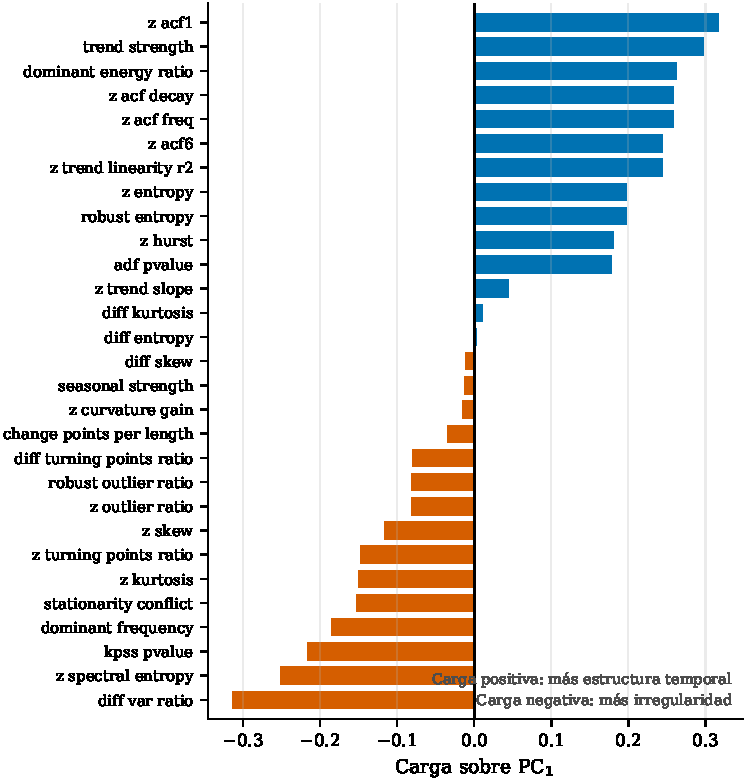
\includegraphics[width=0.62\linewidth]{figuras/fig3_loadings_pc1.pdf}
\caption{Loadings of the 29 features on the first principal component. Positive loadings
correspond to exploitable temporal structure and negative ones to irregularity. The
interpretability of these loadings is what distinguishes the index from a complexity
scalar without a decomposition.}
\label{fig:loadings}
\end{figure}

\paragraph{How much variance the component retains.} $\mathrm{PC}_1$ explains 26.9\% of
the variance of the standardized space of 29 descriptors; $\mathrm{PC}_2$ explains 12.3\%,
and 10 components are needed to reach 80\%. It is worth declaring because it bounds what
the index is and what it is not: \textbf{it is not a faithful representation of the
feature space}, and anyone who uses it to reconstruct the original descriptors will obtain
a poor approximation. It is a scalar summary whose validity rests not on retained variance
but on external criteria ---the correlation with forecast error, the usefulness for
deciding out of sample--- which the following sections test one by one. That 27\% of
variance suffices for both is, in fact, part of the result: the dimension that separates
easy from difficult series is a single one and does not require reconstructing the rest of
the space.

\subsection{The index anticipates forecast error}\label{sec:anticipa}

Over the 99{,}935 series with a computed index, the correlation with the sMAPE of the
naive forecast is $r=0.405$ (Pearson) and $\rho=0.399$ (Spearman). Restricting to the
subset where all four complexity measures are defined ($n=96{,}891$), which is the fair
basis of comparison, $r=0.411$.

Figure~\ref{fig:indice}(a) shows that the relation is monotone across the whole range: the
mean error grows steadily across deciles of the index, from $0.059$ to $0.301$. By
quartiles the values are $0.072$, $0.115$, $0.141$ and $0.236$, a factor of \textbf{3.29}
between the extremes.

\begin{figure}[htbp]
\centering
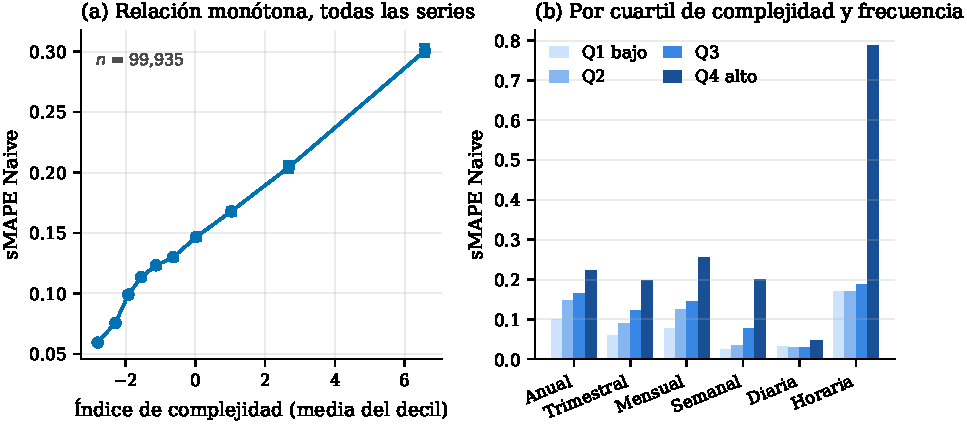
\includegraphics[width=\linewidth]{figuras/fig4_indice_error.pdf}
\caption{(a) Mean error of the naive forecast by decile of the index, with 95\% confidence
intervals. (b) The same analysis by quartile within each frequency. The gradient is steep
in the hourly frequency and practically nonexistent in the daily one.}
\label{fig:indice}
\end{figure}

\subsection{The index is not redundant with the classical measures}\label{sec:redundancia}

Table~\ref{tab:validacion} compares the index with the three established measures. The
result calls for a careful reading: Lempel-Ziv complexity beats the index on rank
correlation ($\rho=0.429$ against $0.399$), while the index beats it on linear correlation
($r=0.411$ against $0.362$). Both statements are true and describe different properties:
LZ orders the series somewhat better, the index models the magnitude of the error better.

\begin{table}[htbp]
\centering
\caption{Correlation with the error of the naive forecast and explained variance
($n=96{,}891$). The $R^{2}$ values come from nested linear regressions on the sMAPE of the
naive forecast.}
\label{tab:validacion}
\begin{tabular}{lccc}
\toprule
\textbf{Measure} & \textbf{Pearson} & \textbf{Spearman} & \textbf{$R^{2}$} \\
\midrule
Complexity index ($\mathrm{PC}_1$)  & \textbf{0.411} & 0.399 & \textbf{0.169} \\
Lempel-Ziv complexity               & 0.362 & \textbf{0.429} & --- \\
Sample entropy                      & 0.240 & 0.275 & --- \\
Permutation entropy                 & 0.054 & 0.062 & --- \\
\midrule
The three classical measures jointly & ---   & ---   & 0.132 \\
Index $+$ classical measures         & ---   & ---   & \textbf{0.183} \\
\bottomrule
\end{tabular}
\end{table}

The regression settles the comparison. The index, as an individual predictor, explains
more variance of the error ($R^{2}=0.169$) than the three classical measures jointly
($R^{2}=0.132$). It is worth being precise about the reach of this claim: it establishes
that the index beats \emph{those three established measures}, not that it is superior to
any complexity characterization or to richer attribute sets. Adding the entropies to the
model with the index improves the fit by 8\%; adding the index to the model with the
entropies improves it by 38\%. The incremental contribution is markedly asymmetric in
favor of the index.

This result is what sustains the contribution: an index built by principal components over
one's own descriptors could be capturing an artifact of the chosen representation, and the
comparison with independent, consolidated measures rules that possibility out.

\paragraph{The index also predicts the error of the best model.} A reasonable objection is
that the index might correlate with the error of the naive forecast through a common cause
---the strength of the trend, say--- without being informative about the difficulty faced
by nontrivial methods. To rule this out we repeat the correlation against the \emph{oracle
error}: the lowest sMAPE among the 27 candidates evaluated, series by series (Table~S9 in
the supplementary material).

The correlation with the oracle error is equal to or higher than the one obtained against
the naive error. The index is not capturing how badly a particular method behaves, but
\emph{how difficult the series is for any available method}, which is the property
relevant to a model assignment decision.

\subsection{How stable the index is}\label{sec:estabilidad}

The index is not reported: it is used to decide. If a series changed stratum under a
perturbation that does not change its nature, the policy would route it differently for
reasons that do not belong to the series. We therefore measured this on 1{,}800 series
---300 per frequency--- recomputing the 29 descriptors on perturbed versions and
projecting them with the same scaler and the same component fitted on the original data,
which is how the index would be used in practice. The quantity that matters is not the
correlation but the \textbf{fraction of series that cross the cut}, because it is the
stratum and not the value that the policy consumes.

\textbf{Against noise the index is stable.} Adding Gaussian noise with standard deviation
proportional to that of the series, 1.4\% of the series change stratum at 1\% noise and
4.8\% at 5\%, with a Spearman correlation that never drops below $0.988$.

\textbf{Against truncation of the history it is not.} Recomputing the index on the last
75\% of the observations, 18.9\% of the series change stratum, and on the last 50\%,
32.6\%, with a Spearman of $0.630$. The first explanation that comes to mind ---that the
effect is mechanical, because length is one of the 29 descriptors--- is ruled out:
repeating everything with an index built without \texttt{log\_length}, the fraction that
changes stratum goes from 32.6\% to 32.3\%. \textbf{It is the shape descriptors that
move}: with half the history, trend strength, seasonal strength and the autocorrelations
describe a different series.

The breakdown by frequency (Table~S5 in the supplementary material) orders the extremes in
a way consistent with the rest of the work: hourly is the most stable (Spearman $0.939$
with half the history) and daily the most fragile ($0.278$), the same order as that of the
index's usefulness. Where there is structure to measure, the measurement is reproducible;
where there is none, the index fits noise. \textbf{The consequence is a condition of use
and not an objection to the instrument}: the index serves to stratify collections whose
series have comparable histories ---the case of M4 and of the decisions evaluated here---
and the stratification must be redone when the available history changes substantially.


\subsection{The dependence on frequency}\label{sec:frecuencia}

The predictive capacity of the index is far from uniform (Figure~\ref{fig:frecuencia}).
The correlation with the error ranges from $r=0.736$ in the hourly frequency to $r=0.019$
in the daily one. Reporting only the aggregate correlation would be misleading: it mixes
six populations with different horizons and dynamics, and the global value may be driven
by differences \emph{between} frequencies rather than \emph{within} them.

\begin{figure}[htbp]
\centering
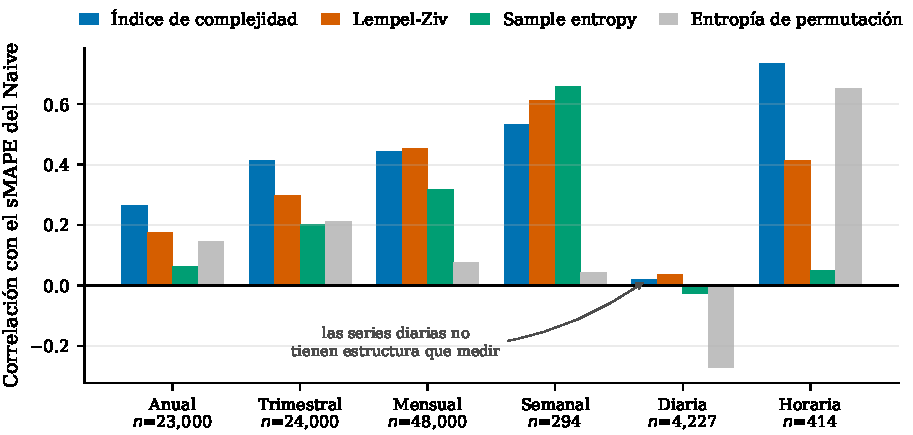
\includegraphics[width=\linewidth]{figuras/fig5_correlacion_frecuencia.pdf}
\caption{Pearson correlation with the sMAPE of the naive forecast, by frequency and by
complexity measure. None of the four measures achieves appreciable signal in the daily
frequency.}
\label{fig:frecuencia}
\end{figure}

The daily case deserves close attention, because at first sight it looks like a failure of
the method. It is not. Three independent pieces of evidence point to those series lacking
exploitable structure:

\begin{enumerate}
\item \textbf{No complexity measure correlates} with the error in that frequency;
      permutation entropy even does so in the negative direction ($-0.273$).
\item \textbf{Clustering barely separates them}: only 1.7\% are assigned to the complex
      group, the lowest proportion of the six frequencies.
\item \textbf{No model beats the benchmark}: ARIMA(1,1,1) obtains $\mathrm{OWA}=1.001$ on
      the daily series and none of the 27 candidates evaluated goes below $0.979$.
\end{enumerate}

Where the index does not discriminate, neither does any forecasting method. The result is
therefore consistent with the hypothesis of the work rather than contradicting it.

\paragraph{External corroboration of the daily case.} The above interpretation ---that the
daily frequency lacks exploitable structure, and not that the index fails to detect
it--- admits a verification independent of this work. The official results of the
competition \cite{m4results} show that \emph{the two winning methods of M4 lose against
the benchmark on the daily series}: Smyl's ES-RNN hybrid obtains OWA $=1.046$ there and
the FFORMA combination $1.019$, both above $1$. Two systems built by specialized teams and
evaluated blind against a hidden test set fall behind a deseasonalized random walk in an
entire frequency. The absence of signal the index reports in the daily frequency therefore
coincides with the absence of signal the competition itself documents.

\subsection{A natural binary partition}\label{sec:clusters}

Figure~S1 in the supplementary material presents the internal validation metrics. The
Silhouette coefficient reaches its maximum at $k=2$ ($0.334$) and the Davies-Bouldin index
its minimum ($1.531$), both with a wide margin over any $k\geq3$. The information criteria
of the Gaussian mixture models decrease monotonically with no elbow, which supports no
partition with more groups. The agreement between geometric and information criteria
reinforces the conclusion.

The resulting partition (Figure~\ref{fig:pca}) separates 79{,}807 regular series (79.9\%)
from 20{,}128 complex ones (20.1\%). Table~\ref{tab:clusters} characterizes them: the
regular group shows a first-lag autocorrelation of $0.923$ against $0.561$, trend strength
of $0.949$ against $0.542$, and a naive forecast error \textbf{116\% higher} in the
complex group.

\begin{figure}[htbp]
\centering
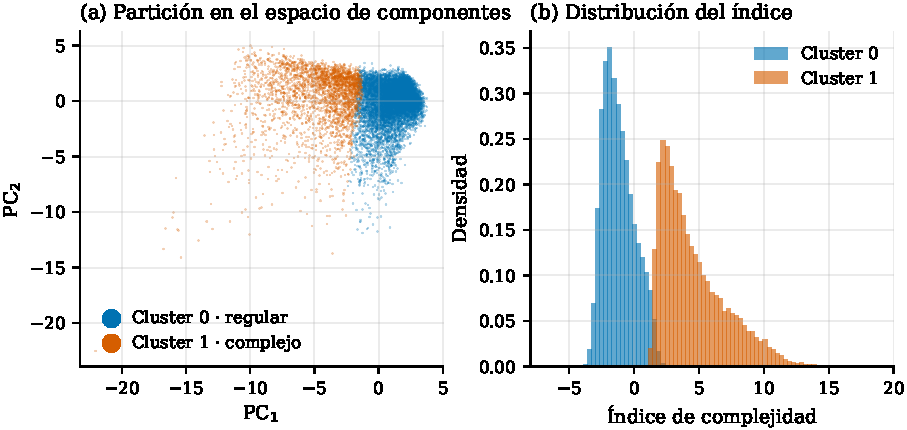
\includegraphics[width=\linewidth]{figuras/fig1_pca_clusters.pdf}
\caption{(a) Projection onto the first two components, with the group assignment
(subsample of 14{,}000 series for legibility). (b) Distribution of the complexity index by
group: the overlap is slight, which indicates that the partition aligns with the axis the
index measures.}
\label{fig:pca}
\end{figure}

\begin{table}[htbp]
\centering
\caption{Characterization of the global groups ($k=2$). The forecast errors are computed
over the 100{,}000 series and the six frequencies.}
\label{tab:clusters}
\begin{tabular}{lrr}
\toprule
\textbf{Feature} & \textbf{Group 0 (regular)} & \textbf{Group 1 (complex)} \\
\midrule
Series                       & 79{,}807 (79.9\%) & 20{,}128 (20.1\%) \\
ACF at lag 1                 & 0.923  & 0.561 \\
STL trend strength           & 0.949  & 0.542 \\
Complexity index (mean)      & $-1.16$ & $+4.60$ \\
sMAPE Naive                  & 0.115  & 0.249 \\
sMAPE ARIMA(1,1,1)           & 0.107  & 0.232 \\
\bottomrule
\end{tabular}
\end{table}

The composition of the groups varies systematically across frequencies: the proportion of
series assigned to the complex group ranges from 1.7\% in daily to 39.1\% in hourly, with
the rest between 15\% and 23\%. On the complete monthly population (48{,}000 series) the
partition reproduces the global pattern (Silhouette $=0.385$, Davies-Bouldin $=1.291$;
split 79.4\% / 20.6\%), with no evidence of a sharper separation than in the full set.

% =====================================================================
\section{The evaluation bank}\label{sec:banco}
% =====================================================================

Every claim about whether a decision rule improves forecasting rests on the metric with
which it is measured. This section builds that bank: it verifies that the implementation
of the benchmark reproduces the one used in the competition, evaluates the bank under the
official metric, and establishes which differences among its members are real and which
are noise. Without this, the experiment of Section~\ref{sec:decision} would have nothing
to be contrasted against.

\subsection{Validation of the evaluation protocol}\label{sec:validacion}

Before comparing models it is necessary to verify that the implementation of the benchmark
reproduces the one of the competition; otherwise every OWA is shifted. Figure~S2 and
Table~S2 in the supplementary material present the comparison against the published values
\cite{makridakis2020}.

The three frequencies with $m=1$ match exactly, which is what one expects: there Naive2
degenerates into the plain naive forecast and no seasonal decomposition intervenes. The
differences in the seasonal frequencies come from the decomposition implementation not
being identical to that of the original code. The global deviation is $0.016$ sMAPE
points.

As an additional check, two independent implementations of the naive forecast ---the one
in the model pipeline and the one in the metrics module--- produce identical values (sMAPE
$14.280$, MASE $3.305$), as do those of the seasonal naive ($12.033$, $2.433$).

\subsection{Evaluation of the bank under OWA}\label{sec:evaluacion}

\textbf{Twenty-eight methods} were evaluated on 5{,}773 series: the three naive benchmarks
of the competition ---Naive, Seasonal Naive and Naive2--- and 25 models distributed across
classical statistical methods (ARIMA, SARIMA, ETS, Holt, Holt-Winters, exponential
smoothing), machine learning (linear regression, LassoLars, Bayesian ridge, SVM, KNN,
Gaussian processes, Random Forest, Bagging, AdaBoost, XGBoost, LightGBM) and hybrid and
neural models (ARIMA-NN, ARIMA-RF, SARIMA-NN, multilayer perceptron, 1D ConvNet, LSTM,
Transformer, LSTM-Conv1D). The policies of Sections~\ref{sec:enrutamiento}
and~\ref{sec:combinar}, and the contrast of Section~\ref{sec:friedman}, operate on
\textbf{27} of those 28: Holt-Winters is excluded because it is undefined where $m=1$ and
the design requires every candidate to be available in every series.

The OWA values are reported reweighted to the actual M4 population, because the evaluated
sample over-represents the daily and hourly frequencies (17.3\% and 7.2\%, against 4.2\%
and 0.4\% in the competition), which are precisely the ones where several models go out of
control. The reweighting is applied separately to sMAPE and MASE before the ratio,
consistently with (\ref{eq:owa}).

Only six models beat the benchmark (Figure~S5 in the supplementary material).
ARIMA(1,1,1) leads with $\mathrm{OWA}=0.932$, followed by SARIMA ($0.934$), LassoLars
($0.973$), linear regression ($0.979$), ETS ($0.993$) and Holt-Winters ($0.995$). The
result reproduces, on a reduced scale, one of the central findings of M4: classical
statistical methods remain competitive against considerably more expensive machine
learning alternatives.

\subsection{The inversion in the hourly frequency}\label{sec:horaria}

The global ordering hides a complete inversion. Figure~\ref{fig:heatmap} shows the OWA of
each model broken down by frequency.

\begin{figure}[htbp]
\centering
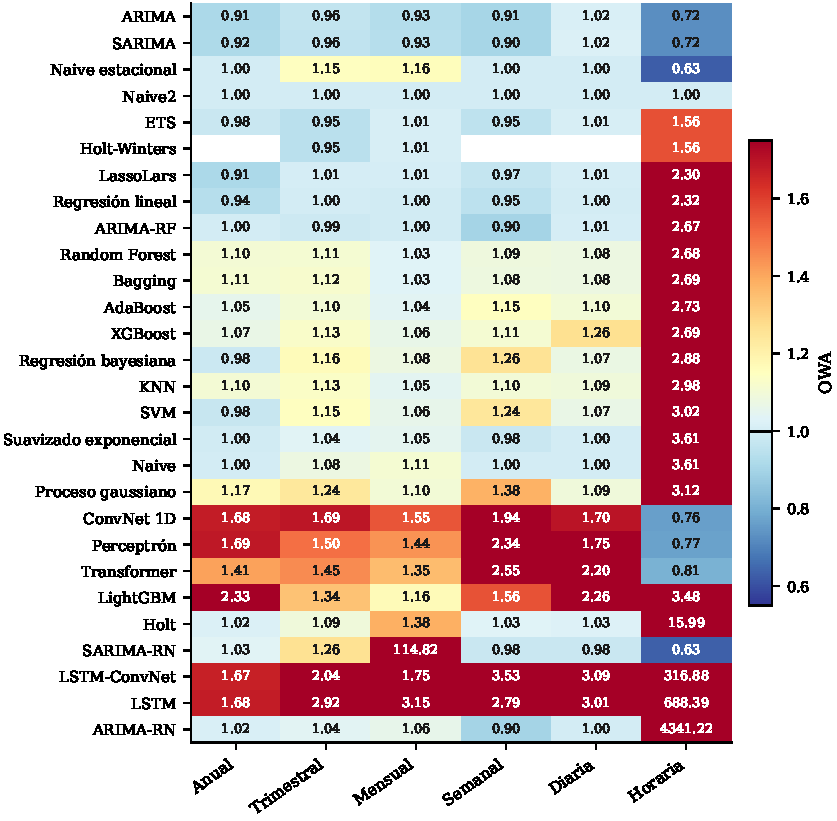
\includegraphics[width=0.72\linewidth]{figuras/fig7_owa_heatmap.pdf}
\caption{OWA by model and frequency. The values shown are exact; the \emph{color scale}
saturates outside the range $[0.55,\,1.75]$ so that the relevant differences remain
distinguishable despite the extreme values of the models that diverge (Table~S3 in the
supplementary material). The black line in the color bar marks the benchmark. Blank cells
correspond to Holt-Winters in the frequencies with $m=1$, where the model does not apply.
The neural networks move from the worst positions to the best only in the hourly
frequency.}
\label{fig:heatmap}
\end{figure}

In the hourly frequency the ordering is completely rearranged. The seasonal naive obtains
the best result of the entire evaluation ($0.626$), followed by SARIMA-NN ($0.631$) and by
ARIMA and SARIMA (both $0.724$). The neural networks, which in the other five frequencies
occupy the last positions with OWA between $1.4$ and $1.7$, sit here below the benchmark
---1D ConvNet $0.762$, perceptron $0.768$, Transformer $0.807$---: the same model that is
60\% worse than Naive2 in the global average beats it by 24\% here. The explanation is
data availability: with $m=24$, 960 observations per series and a marked daily cycle,
these architectures have enough to learn the pattern, and in the remaining frequencies
---median length between 29 and 202 observations--- they do not. It is precisely the kind
of phenomenon that a structure-conditioned selection can exploit and that an aggregate
evaluation would not let one see.

\subsection{Two failure modes the average hides}\label{sec:extremos}

Four models show OWA between 11 and 365, figures that at first sight suggest unusable
performance but whose medians sit between $0.9$ and $1.8$. The average is dominated by a
handful of series, and the mechanism is an asymmetry between the two metrics that make up
OWA: \textbf{sMAPE is bounded at 200 and MASE has no upper bound}, so a forecast that
diverges saturates in the former and drags the average of the latter without limit. The
witness case is series \texttt{H366}, with sMAPE $=199.99$ and MASE $=127{,}224$.

To that failure mode ---typically correct, catastrophic in a few series--- is added a
different one, worth separating because it reads differently: LightGBM, the worst of the
bank, fails in the \emph{center} of the distribution and for a structural reason, since a
tree ensemble predicts averages of leaves and cannot extrapolate outside the observed
range. In yearly it issues a flat forecast in 95.7\% of the series.

\textbf{The distinction between a badly fitted model and one structurally inadequate for a
family of series is exactly the kind of heterogeneity that a structure-conditioned rule
ought to capture}, and it explains why LightGBM never appears in the sets that
Section~\ref{sec:combinar} selects for yearly or hourly. The practical implication is that
when reporting mean MASE it is advisable to accompany it with the median and the count of
extreme cases. The full breakdown, with the per-model table and the diagnosis of LightGBM
frequency by frequency, is in Section~S2 of the supplementary material.

\subsection{Statistical significance of the differences}\label{sec:friedman}

The comparisons above rest on averages, which Section~\ref{sec:extremos} showed to be
fragile. To contrast the differences without that fragility we apply the standard
procedure for comparing multiple methods over multiple data sets \cite{demsar2006}: models
are ranked \emph{within each series}, the hypothesis that all perform equally is tested
with Friedman, and the pairs that differ are identified with the Nemenyi post-hoc. A
rank-based analysis is immune to the problem of the previous subsection, because only the
order within each series matters and not how far the worst forecast strays. The design
requires every model to be evaluated on every series: Holt-Winters is excluded because it
does not apply where $m=1$, and 26 series are discarded because some fit failed to
converge, which leaves $k=27$ models over $N=4{,}747$ series.

Friedman rejects equivalence with room to spare ($\chi^{2}=13{,}167$, $p<10^{-15}$) and
the Nemenyi critical difference at 5\% is $0.602$ rank positions.

\begin{figure}[htbp]
\centering
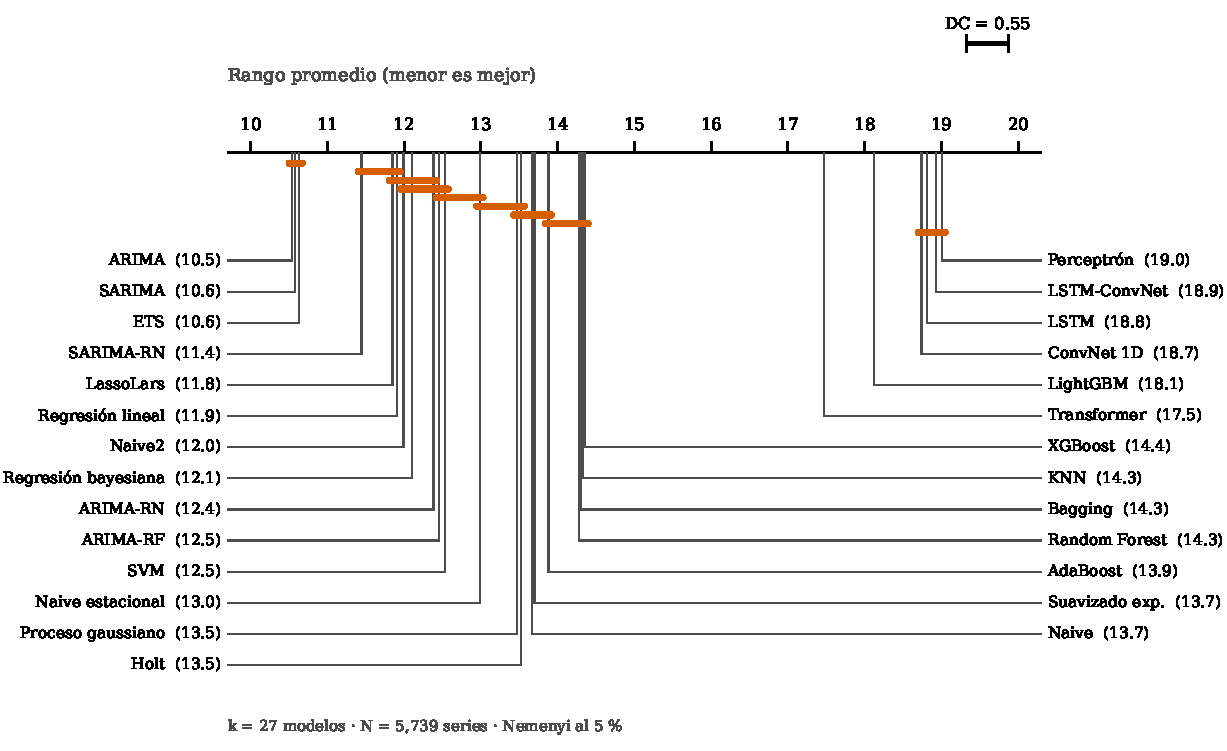
\includegraphics[width=\linewidth]{figuras/fig10_nemenyi.pdf}
\caption{Critical difference diagram. Each model sits at its mean rank over the 4{,}747
series; lower is better. The horizontal bars join groups whose differences do not reach
the critical difference, that is, models statistically indistinguishable from one
another.}
\label{fig:nemenyi}
\end{figure}

Three results deserve attention.

\paragraph{There is a statistical tie at the top.} ARIMA ($10.55$), SARIMA ($10.58$) and
ETS ($10.67$) fall within the critical difference: their differences are not significant.
The ordering by OWA ---which placed ETS sixth, behind two regression methods--- suggested
a hierarchy the test does not support. The defensible conclusion is not that ARIMA is the
best model, but that \emph{the three classical statistical methods are equivalent to one
another and superior to the rest}.

\paragraph{The models that diverge are not bad: they are unstable.} SARIMA-NN moves from
last place by OWA ($31.06$) to \textbf{fourth} by ranks ($11.25$), indistinguishable from
ETS. ARIMA-NN moves from 29th by OWA ($23.45$) to ninth by ranks ($12.46$). Their
\emph{typical} behavior is competitive; what sinks them in the average are a few series
where the forecast blows up. Both readings are correct and describe different phenomena:
the average measures tail risk, the rank measures habitual performance. Reporting both is
what makes it possible to tell a consistently mediocre model from one that is usually good
but occasionally catastrophic ---a distinction neither metric reveals on its own.

\paragraph{The neural networks come last by ranks too.} 1D ConvNet, perceptron and LSTM
occupy the final positions with ranks between $18.5$ and $18.9$, well beyond the critical
difference with respect to any classical method. Unlike the previous case, here the poor
performance is not an artifact of the average: it is systematic, series by series.

The analysis was repeated using MASE instead of sMAPE to build the ranks. The two
orderings are practically identical (Spearman correlation $=1.000$; no model moves more
than one position), which indicates that the conclusions do not depend on the metric
chosen to rank.

% =====================================================================
\section{What decision structure supports}\label{sec:decision}
% =====================================================================

The two preceding sections establish that the index \emph{correlates} with forecasting
difficulty and that there is a bank of 27 candidates measured with the official metric.
Neither establishes that the index is \emph{useful}, which is a different and more
demanding claim: that using it improves a concrete decision, evaluated out of sample. This
section tests it, and then does what is rarely done with a favorable result: it measures
how far the optimum still is, checks whether the shortfall is due to the scalar summary or
to the approach, and ends by identifying the cause of the limit.

\subsection{Is the index useful for choosing a model?}\label{sec:enrutamiento}

The previous results establish that the index \emph{correlates} with forecasting
difficulty. They do not establish that \emph{using} it improves a decision, which is a
different and more demanding claim. This section tests it directly.

\paragraph{Design.} A routing rule is a function that assigns a model to each series. The
number of complexity strata is fixed \textbf{a priori at two}, justified by the cluster
analysis of Section~\ref{sec:clusters}, which identifies $k=2$ through internal criteria
without observing any forecast error. That choice is therefore independent of the
experiment that follows: it is not selected by looking at performance on the test set. The
sweep over other values is reported below as a robustness analysis, not as a selection
criterion.

Four rules are compared:

\begin{description}
\item[A · Fixed] a single model for the whole collection, the best one in training.
\item[B · By frequency] the best model of each frequency.
\item[C · By index] the best model of each (frequency, complexity stratum) pair.
\item[D · Oracle] the best model for each individual series. It is not attainable by any
      real rule; it is reported as an upper bound.
\end{description}

Each rule is \textbf{learned} on half of the series and \textbf{evaluated} on the other
half, with the partition stratified by frequency and repeated over 30 random splits. The
stratum cuts are computed using the training set only and applied to the test set; using
the quantiles of the full set would introduce information leakage. The experiment refits
no model: it reuses the per-series errors already computed.

\textbf{Policy B is the control that gives the result its validity.} The relevant question
is not whether routing helps ---evidently it does--- but whether the index contributes
anything above what the frequency, known in advance and at no cost, already provides.

\begin{table}[htbp]
\centering
\caption{Performance of the routing rules on the test set. Mean and standard deviation
over 30 random splits, with two complexity strata per frequency.}
\label{tab:enrutamiento}
\begin{tabular}{llrr}
\toprule
& \textbf{Rule} & \textbf{OWA} & \textbf{S.d.} \\
\midrule
A & One fixed model for the whole collection      & 0.9234 & 0.0083 \\
B & The best model of each frequency              & 0.9140 & 0.0070 \\
C & \textbf{The best of each frequency and stratum} & \textbf{0.8835} & 0.0057 \\
\midrule
D & Per-series oracle (unattainable bound)        & 0.5423 & 0.0038 \\
\bottomrule
\end{tabular}
\end{table}

\paragraph{Result.} The index-based policy beats the frequency-only policy in \textbf{all
30 splits}, with a mean advantage of $0.0306$ OWA points and a paired Wilcoxon test of
$p = 1.9\times10^{-9}$ (Table~\ref{tab:enrutamiento},
Figure~\ref{fig:enrutamiento}a). Expressed over the distance between the fixed model and
the oracle, frequency alone closes 2.4\% and frequency together with the index closes
10.5\%: four times as much.

\begin{figure}[htbp]
\centering
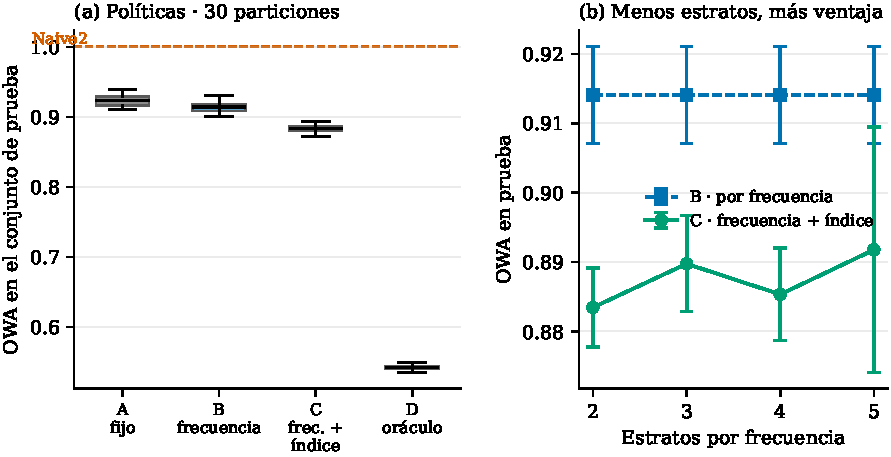
\includegraphics[width=\linewidth]{figuras/fig11_enrutamiento.pdf}
\caption{(a) OWA of each rule on the test set, over 30 random splits. (b) Effect of the
number of complexity strata: the advantage of the index over frequency-based routing is
significant in every case, but decreases monotonically as granularity increases.}
\label{fig:enrutamiento}
\end{figure}

\paragraph{Robustness to the number of strata.} Repeating the experiment with three, four
and five strata leaves the advantage over frequency-based routing significant in all four
cases, so the result does not depend on the chosen granularity; the magnitude decreases
monotonically, which is to be expected because with more strata each rule is estimated on
fewer series. The value fixed a priori ---two strata, taken from the cluster analysis---
turns out to be the best performing out of sample as well, with an advantage of $+0.0306$
against $+0.0243$, $+0.0287$ and $+0.0223$ for the other granularities. The full sweep is
in Table~S4 of the supplementary material.

This result admits a reading that goes beyond the experiment, but it is worth stating
precisely. The cluster analysis of Section~\ref{sec:clusters} identifies $k=2$ through
internal criteria ---Silhouette, Davies-Bouldin, AIC and BIC--- without observing any
forecast error; the routing experiment identifies two strata as the optimal granularity by
observing only out-of-sample performance. \textbf{Two independent procedures therefore
agree that the exploitable structure is binary}, one through the geometry of the feature
space and the other through the quality of the decisions that space enables.

\textbf{What must not be claimed is that they are the same partition}, and the direct
check rules it out: the cluster splits the 99{,}935 series into 20{,}128 and 79{,}807,
while the median cut of the index splits them into halves by construction, and the two
assignments agree on 70.1\% of the series against the 50\% chance would give. The relation
between them is not one of identity but of partial inclusion: the minority cluster falls
\emph{entirely} inside the high-complexity stratum, without a single exception, so that it
identifies a core of the difficult extreme and not its full half. What the two procedures
share is the cardinality of the useful partition, not its boundary.

\paragraph{What the index does not capture, and what that gap really measures.} The
index-based rule closes 10.5\% of the distance to the oracle. There is therefore
predictive information at the individual series level that a scalar built by principal
components does not manage to represent.

It is worth being precise about what the remaining 89.5\% is, because the immediate
reading ---that this fraction is available and the index fails to exploit it---
overestimates what any policy could recover. The oracle chooses, series by series and
looking at the test set, the best of the 27 candidates. The distance separating it from
the fixed model therefore mixes two things the metric does not distinguish: the selection
information the features do not capture, and the error that \emph{no} model in the bank
could have avoided in that series. Only the first is recoverable, and the experiment does
not separate it from the second. \textbf{The 89.5\% is therefore an upper bound on what is
left to gain, not a measure of wasted signal}, and the same caveat applies to the other
gap fractions reported in this work. What the comparison with the meta-learner of
Section~\ref{sec:meta} does establish, and does not depend on this ambiguity, is that the
fraction recoverable \emph{by structural features} is practically exhausted:
twenty-nine attributes do not get much further than one.


\paragraph{How aggregation is done, and why it is declared.} The policy experiments of
this section average the error over the series of the sample, whereas the model evaluation
of Section~\ref{sec:evaluacion} weights each frequency by its share of the full
collection. Both aggregations are legitimate and answer different questions ---performance
over the series actually evaluated, and expected performance over M4--- but they are not
interchangeable: the sample over-represents the daily and hourly frequencies, which weigh
21\% and 8.7\% in it against 4.2\% and 0.4\% in the collection. For the comparisons
between policies in this section the choice alters no conclusion ---combining beats
choosing under both aggregations and in five of the six frequencies separately--- but it
does in Section~\ref{sec:nbeats}, where both are reported explicitly.

\subsection{How much is lost against a full meta-learner?}\label{sec:meta}

The rule of the previous subsection uses a scalar and two strata. The feature-based model
selection literature ---FFORMS \cite{talagala2018} and FFORMA \cite{monteromanso2020}---
uses the full attribute vector and a trained meta-model. The pertinent question is not
which wins in the abstract, but \emph{how much the simplification costs}.

\paragraph{What can and cannot be compared.} FFORMA is not reproducible with these data:
it combines \emph{forecasts} with learned weights, and the available record stores the
error per series and model, not the predictions of its base ensemble, which moreover comes
from a different pool of methods. Quoting its published OWA of 0.838 over the full M4 and
contrasting it with 0.884 over 5{,}773 series would be misleading: different set,
different pool, different task. What is legitimate is to implement the \emph{approach} on
the same data, the same pool and the same partition protocol:

\begin{itemize}
\item[\textbf{E}] \textbf{Classifier} (FFORMS style): a random forest over the 29
      attributes predicts which model wins in each series.
\item[\textbf{F}] \textbf{Per-model regressor} (FFORMPP style): one random forest per
      model predicts its $\log(1+\mathrm{sMAPE})$ and the one with the lowest predicted
      error is chosen.
\item[\textbf{E$'$}] \textbf{The same classifier with the right loss}: the model chosen is
      the one that minimizes expected regret under the forest's probabilities, instead of
      the most probable class. It is added by the diagnosis below.
\end{itemize}

\begin{table}[htbp]
\centering
\caption{The index against meta-learning over the full vector of 29 attributes. Same data,
same pool, same 30 splits.}
\label{tab:meta}
\begin{tabular}{llrr}
\toprule
& \textbf{Policy} & \textbf{OWA} & \textbf{Closes} \\
\midrule
A & Global fixed model & 0.9234 & --- \\
B & By frequency & 0.9140 & 2.4\% \\
C & Frequency $\times$ index (2 strata) & \textbf{0.8835} & 10.5\% \\
E & Classifier, 29 attributes & 1.4927 & $-152.2$\% \\
E$'$ & Classifier with costs, 29 attributes & \textbf{0.8661} & \textbf{15.0}\% \\
F & Per-model regressor, 29 attributes & 0.8746 & 12.8\% \\
D & Per-series oracle (bound) & 0.5423 & 100\% \\
\bottomrule
\end{tabular}
\end{table}

\begin{figure}[htbp]
\centering
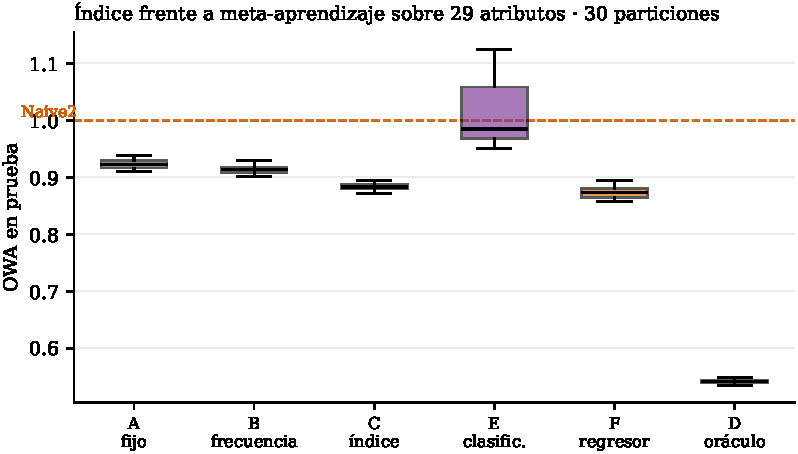
\includegraphics[width=\linewidth]{figuras/fig12_metaaprendizaje.pdf}
\caption{Distribution of the OWA of each policy over the 30 splits. The box of the
classifier (E) falls outside the range of the plot in several splits; its dispersion
---standard deviation of 2.59 against 0.006 for the index--- is as informative as its
mean. E$'$ is the same classifier decided with the right loss.}
\label{fig:meta}
\end{figure}

The result in Table~\ref{tab:meta} and Figure~\ref{fig:meta} has two readings and neither
is comfortable for an extreme position.

\paragraph{The full apparatus does improve on the index, and it is worth saying by how
much.} Policy F reaches 0.8746 against 0.8835 for the index ---an advantage of 0.0089,
$p=7.9\times10^{-5}$, with the index ahead in 4 of the 30 splits--- and the best of all is
E$'$, at 0.8661. Against it, what the full apparatus buys over the scalar is 0.0174: four
and a half points of the journey toward the oracle. The argument in favor of the index is
therefore not that it matches the apparatus, but that it recovers seven tenths of what the
apparatus achieves using a scalar and a median cut, and that the 85\% neither of them
reaches is the same. Section~\ref{sec:dospasos} returns to the comparison under a protocol
that combines as well as chooses, and finds an advantage of $0.0091$ with $k=1$ that
vanishes with five.

\paragraph{The classifier fails, and not for the reason it seems.} Policy E lands at
1.4927, worse than not routing at all, with a standard deviation of 2.59 across splits.
The immediate reading is that the label ---\emph{which} model wins in this series--- is
noise, in line with Section~\ref{sec:semillas}. Section~S3 of the supplementary material
puts it to the test against the other three available explanations, on the same splits and
the same forest, and forces a qualification. Class imbalance is not the cause: correcting
it worsens the typical split and only trims the tail. The label, on the other hand, is
indeed close to arbitrary ---in 11.5\% of the series the first and second have the
\emph{same} sMAPE--- and caps accuracy at 18.5\%. But that is not what produces the 1.49.
What produces it is that classification minimizes the $0$--$1$ loss while the real cost of
being wrong ranges from thousandths to orders of magnitude: the worst 1\% of the series
contributes 40\% of the excess. \textbf{Keeping the same forest and the same label, and
changing only the decision rule to the one that minimizes expected regret, OWA goes from
1.4927 to 0.8661} ---policy E$'$---, better than the index in all 30 splits and better
than the regressor in 22 of 30. The warning for anyone implementing feature-based
selection survives with a different reason: predicting the winner and trusting it is
fragile, but not because the label is noise ---the regressor uses the same one--- but
because that formulation discards the cost structure.


\subsection{Is the limit in the characterization or in choosing?}\label{sec:combinar}

The two preceding subsections share an assumption that was not made explicit: that
characterization serves to \emph{choose} a model. Policies B, C, E and F assign one method
to each series and discard the rest. There is a concrete reason to doubt that this is the
right use of characterization: FFORMA \cite{monteromanso2020} placed second in M4 with OWA
$=0.838$ also using series attributes, but \emph{combining} the forecasts of nine methods
with learned weights, without choosing any. If the measured ceiling belonged to the
approach, that result should not exist.

\paragraph{Design.} Two families of policies that combine instead of choosing are added to
the same protocol. For each split and each stratum, models are ranked by OWA \emph{in
training} and the top $k$ are averaged over the test series; the simple average is
deliberate, because it is the most austere form of combination there is and the one the
competition itself uses as a benchmark. Family $B_k$ combines within each frequency and
family $G_k$ within each frequency $\times$ complexity stratum. With $k=1$ both reduce to
policies B and C already seen, so that the comparison is continuous.

\begin{table}[htbp]
\centering
\caption{Choosing one model against combining $k$. The contribution column is the
difference between combining by frequency and combining by frequency $\times$ stratum: it
measures what the index adds at an equal number of combined models.}
\label{tab:combinar}
\begin{tabular}{crrrcr}
\toprule
$k$ & \textbf{$B_k$} & \textbf{$G_k$} & \textbf{Index} &
\textbf{$G$ better} & \textbf{$p$} \\
  & \textbf{frequency} & \textbf{freq.$\times$index} & \textbf{contribution} & & \\
\midrule
1 & 0.9187 & 0.8869 & $+0.0318$ & 30/30 & $1.9\times10^{-9}$ \\
2 & 0.8951 & 0.8787 & $+0.0165$ & 20/30 & $6.1\times10^{-4}$ \\
3 & 0.8761 & 0.8688 & $+0.0073$ & 26/30 & $3.9\times10^{-7}$ \\
4 & 0.8745 & 0.8672 & $+0.0073$ & 27/30 & $2.0\times10^{-7}$ \\
5 & \textbf{0.8725} & \textbf{0.8647} & $+0.0078$ & 25/30 & $4.4\times10^{-6}$ \\
\midrule
\multicolumn{2}{l}{Per-series oracle (bound)} & 0.5448 & & & \\
\bottomrule
\end{tabular}
\end{table}

\paragraph{Why $B_1$ does not coincide with policy B of
Section~\ref{sec:enrutamiento}.} Both pick the best model of each frequency over the same
5{,}674 series and the same bank, with metrics that agree digit by digit, yet $B_1$ gives
$0.9187$ and B gave $0.9140$. The difference is one of \emph{partitioning}: there each
frequency is split into exact halves and here each series is assigned by an independent
draw, so that the training size fluctuates. Repeating B under both schemes on the same
data yields $0.9141$ and $0.9181$, which reproduces the gap. \textbf{The figures are
comparable within each experiment and not across them.}

Table~\ref{tab:combinar} and Figure~\ref{fig:combinar} contain three results.

\paragraph{The two decisions weigh the same, and it is advisable to claim no more than
that.} Going from choosing one model to averaging five improves OWA by $0.0462$ within the
frequency-based policy and by $0.0222$ within the index-based one. The contribution of the
index over frequency, which Section~\ref{sec:enrutamiento} presented as the central
result, is $0.0318$. The two quantities are of the same order, and the temptation to
declare one of them the winner does not survive sampling error: a bootstrap that resamples
series within each frequency and averages over splits places the gain from combining at
$+0.0267$ (95\% CI $[+0.0143,\ +0.0393]$) and that from stratifying at $+0.0214$
($[+0.0110,\ +0.0328]$). \textbf{Both are significant separately; their difference,
$+0.0053$ with interval $[-0.0148,\ +0.0254]$, is not.} What the evidence supports is that
these are two decisions of comparable magnitude, and that the feature-based forecasting
literature attends to only one of them.

\paragraph{The contribution of the index decays as models are combined, until it is no
longer detectable.} $G_k$ beats $B_k$ for every $k$ evaluated, but the magnitude decreases
monotonically and the evidence supporting it runs out before the series of point estimates
does. With a resampling of \emph{series} ---the unit that corresponds, as argued below---
the contribution is $+0.0215$ with interval $[+0.0110,\ +0.0326]$ when choosing one model
and $+0.0131$ with $[+0.0022,\ +0.0233]$ when combining two, both clearly above zero. From
there on the intervals contain it: $+0.0055$ with $[-0.0024,\ +0.0139]$ for $k=3$,
$+0.0018$ with $[-0.0056,\ +0.0098]$ for $k=4$ and $+0.0042$ with $[-0.0043,\ +0.0120]$
for $k=5$.

\textbf{The defensible reading is that combination absorbs what stratification used to
solve, up to a point where the contribution of the index is no longer distinguishable from
zero.} It is established where the policy \emph{chooses}, and it is not at the ensemble
sizes this section finds best. Saying that characterization \emph{relocates} toward
deciding what to combine would go beyond what these data allow: what they show is that its
usefulness is greatest when selecting and dilutes when combining.

\paragraph{And the ceiling is still low.} The best policy evaluated, $G_5$, reaches
$0.8647$ and closes 14.4\% of the distance between the frequency control and the
per-series oracle, against 8.5\% for the policy that chooses. The contribution grows, and
even so the bulk of that distance ---with the caveat about its interpretation introduced
in Section~\ref{sec:enrutamiento}--- goes unclosed. The conclusion of
Section~\ref{sec:meta} holds with one important correction: the limit comes neither from
having summarized structure in a scalar \emph{nor} from having chosen instead of combined,
because correcting the latter barely doubles a contribution that remains small.

\begin{figure}[htbp]
\centering
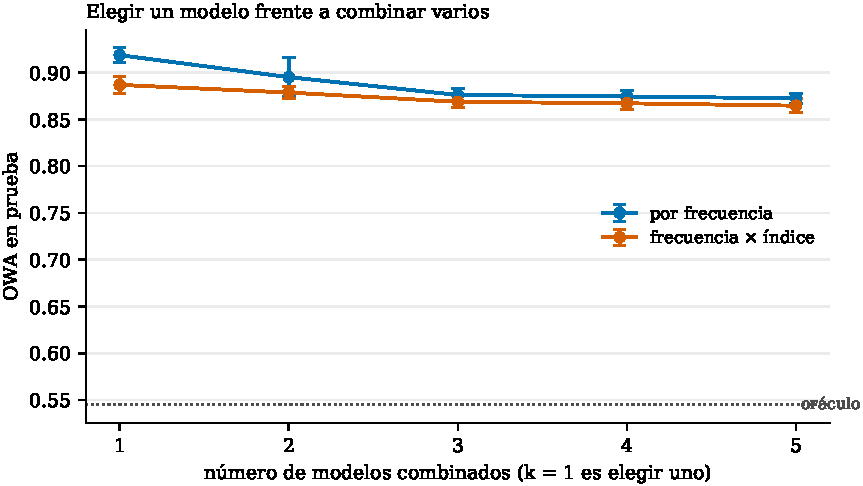
\includegraphics[width=0.82\linewidth]{figuras/fig13_combinar.pdf}
\caption{Test OWA as a function of how many models are combined, with standard deviation
over the 30 splits. At $k=1$ both curves are policies B and C. The separation between
curves is the contribution of the index; the slope of each curve is the contribution of
combining.}
\label{fig:combinar}
\end{figure}

\paragraph{Control: averaging is not enough, one has to know what to average.} The
immediate objection to the above is that the merit belongs to the average and not to the
information that decides what to average. Table~\ref{tab:controles} answers it. Averaging
five models drawn at random from the bank produces OWA $=5.60$, a predictable disaster
because the bank contains models that diverge. The demanding control is the second one:
drawing five \emph{from among the ten best in training} ---thereby eliminating the easy
explanation--- still leaves OWA $=1.26$ against $0.870$ for the five best. Knowing the
fine ordering is worth $0.39$ OWA points, in all 30 splits. \textbf{Combination does not
replace characterization: it needs it.}

\begin{table}[htbp]
\centering
\caption{Controls on the combination policy. The first asks whether averaging suffices;
the second, whether $k=5$ is tuned to the test set.}
\label{tab:controles}
\begin{tabular}{lr}
\toprule
\textbf{Policy} & \textbf{OWA} \\
\midrule
\multicolumn{2}{l}{\emph{Is averaging enough?}} \\
\quad 5 models at random from the full bank & 5.60 \\
\quad 5 at random from among the 10 best in training & 1.26 \\
\quad \textbf{the 5 best in training} & \textbf{0.870} \\
\midrule
\multicolumn{2}{l}{\emph{Is $k=5$ tuned to the test set?}} \\
\quad $k$ fixed at 5 & 0.870 \\
\quad \textbf{$k$ chosen in training, by frequency} & \textbf{0.868} \\
\bottomrule
\end{tabular}
\end{table}

\paragraph{The number of models is not tuned to the test set.} Fixing $k=5$ because it is
the best value observed on the test set would be the same shortcut this work rejects
elsewhere. A policy was therefore implemented that chooses $k$ \emph{within the training
half} and by frequency, and its performance is \emph{better} than that of fixed $k$
($0.868$ against $0.870$), so the choice does not introduce overfitting but avoids it. The
values it selects are interpretable: five in yearly and monthly, four in quarterly and
hourly, two in weekly and \textbf{one in daily}. That the frequency without exploitable
structure (Section~\ref{sec:frecuencia}) is also the only one where the rule decides not
to combine is a coherence check that was not sought.

\paragraph{The set being combined is unstable, and that confirms the mechanism.} One
possible objection is that the comparison favors combination if the set of the five best
varies across splits. Two things should be separated. The comparison is symmetric in
information: both policies observe \emph{only} the training half, and the difference lies
in how many models they carry from there to the test, not in what they know. But the
instability does exist and deserves reporting: the mean Jaccard similarity of the set of
five across splits ranges from $0.34$ in daily to $0.71$ in hourly, with values around
$0.45$ elsewhere; that is, close to half the members change from one split to another. Far
from weakening the result, that instability \emph{is} the mechanism: if the ordering of
models were stable, keeping the first would be a safe decision. It is not, and that is why
averaging five turns out to be more robust than betting on one. It is the same instability
Section~\ref{sec:semillas} measures directly, and the reason the classifier of
Section~\ref{sec:meta} fails to identify the winner ---although, as seen there, that is
not what sinks its OWA.

\paragraph{What is resampled, and why it changes the conclusion.} The 30 splits are not 30
independent samples: they are re-divisions of the same 5{,}674 series. A test that treats
them as replicates ---a Wilcoxon test over splits, or a \emph{bootstrap} that resamples
those 30 differences--- answers whether the contribution is \emph{consistent} under
re-splitting this sample, which is a statement of internal reproducibility and is valid as
such. It does not answer whether the contribution would survive having drawn other series,
which is what is needed in order to generalize, and that is why it produces intervals that
are too narrow.

Resampling series within each frequency and averaging over splits within each replicate,
the intervals come out \textbf{between three and six times wider} than those obtained by
resampling splits, and three of the five come to contain zero. The figures in the previous
paragraph are those of this procedure. The split-based test is kept where it belongs
---to claim consistency, not significance--- and is declared as such.

\paragraph{Coherence with FFORMA.} The result reconciles the measured ceiling with
FFORMA's second place rather than contradicting it. Averaging five models with equal
weights within two strata reaches $0.8647$; FFORMA combines nine with learned weights and
reaches $0.838$ over the full collection. Both values belong to the same regime, and the
difference between them is attributable to the sophistication of the weights and of the
pool, not to a change of approach. What the evidence of this work rules out is not the use
of series features, but their use \emph{for selecting}, which is precisely what FFORMA
does not do and what the classifier variant (Section~\ref{sec:meta}) takes to the extreme.

\paragraph{Does anything depend on these 29 descriptors in particular?} The set was
chosen for interpretability and coverage of families, not by a selection procedure, and
one may ask how much of the above depends on that choice. The canonical reference is
catch22 \cite{lubba2019}, 22 features filtered from the 4{,}791 of hctsa by classification
performance and mutual redundancy. An analogous index was built ---the negative of the
first principal component over the 22 standardized features, with the sign fixed using the
training half only--- and submitted to the same tests.

\begin{table}[htbp]
\centering
\caption{The index of this work against one built on catch22, under the same protocol of
30 splits. OWA values; lower is better.}
\label{tab:catch22}
\begin{tabular}{crrrr}
\toprule
$k$ & \textbf{Own index} & \textbf{catch22} & \textbf{Difference} & \textbf{$p$} \\
\midrule
1 & 0.8802 & 0.8793 & $-0.0008$ & $0.25$ \\
2 & 0.8744 & \textbf{0.8710} & $-0.0034$ & $7.1\times10^{-5}$ \\
3 & 0.8637 & \textbf{0.8614} & $-0.0023$ & $3.2\times10^{-3}$ \\
4 & 0.8607 & 0.8602 & $-0.0005$ & $0.31$ \\
5 & 0.8592 & \textbf{0.8543} & $-0.0049$ & $8.9\times10^{-5}$ \\
\bottomrule
\end{tabular}
\end{table}

\textbf{The canonical set performs at least as well as our own.} catch22 ties at $k=1$ and
$k=4$ and beats the own index in the other three, always by margins no larger than $0.005$
of OWA. The sense of the result does not change because of this, and if anything it is
reinforced: a feature set built by the opposite criterion ---automatic filtering by
classification performance over 93 collections, rather than selection by
interpretability--- opens no margin that the own index was leaving unused. In correlation
with the error of the naive forecast the split is also even ---catch22 is better in
monthly, weekly and daily; the own index in quarterly, hourly and yearly. The conclusion
is best stated plainly: the 29 descriptors are not the source of the result, and neither
would 22 selected by a different procedure be. Far from weakening the work, this
reinforces its thesis: if two characterizations built on opposite criteria perform the
same, it is because the margin available to characterization is narrow, and what decides
lies elsewhere.

\subsection{Against a published meta-learner}\label{sec:dospasos}

Section~\ref{sec:meta} compared the index against two in-house formulations of
meta-learning, but not against a published method. The most pertinent is the two-step
scheme of Vaiciukynas and co-authors \cite{vaiciukynas2021}, which on M4 data trains one
meta-learner to \emph{rank} the methods and a second one to predict the \emph{size} of the
ensemble for each series. It is exactly the per-series generalization of the rule of
Section~\ref{sec:combinar}, which ranks and fixes the size per stratum.

\paragraph{Why quoting their figure is not enough.} That work reports sMAPE $=9.21$ on M4,
but evaluated on 12{,}561 microeconomic series and not on the 100{,}000: its reference
Theta gives $11.05$ where the official Theta of the competition gives $12.309$. These are
different scales, and putting them in the same table would mislead just as with FFORMA.
What is informative is to implement the approach on these data, this pool and this
protocol. Step 1 trains one random forest per model that predicts its
$\log(1+\mathrm{sMAPE})$ from the 29 attributes, pooling the six frequencies, and ranks
the models of each series by predicted error; step 2 trains another forest that predicts
the optimal $k$ for each series.

\begin{table}[htbp]
\centering
\caption{The two-stratum index against per-series ranking with the 29 attributes, at an
equal number of combined models. Thirty splits.}
\label{tab:dospasos}
\begin{tabular}{crrrr}
\toprule
$k$ & \textbf{Index} & \textbf{Meta-learner} & \textbf{Difference} & \textbf{$p$} \\
  & \textbf{2 strata} & \textbf{29 attributes} & & \\
\midrule
1 & 0.8823 & 0.8855 & $+0.0032$ & $0.84$ \\
2 & 0.8769 & \textbf{0.8682} & $-0.0086$ & $0.014$ \\
3 & 0.8683 & \textbf{0.8613} & $-0.0070$ & $0.015$ \\
4 & 0.8665 & 0.8614 & $-0.0052$ & $0.097$ \\
5 & 0.8625 & 0.8655 & $+0.0030$ & $0.18$ \\
\midrule
\multicolumn{5}{l}{\emph{Full two-step scheme, with $k$ learned per series:}
  0.8647 \quad ($p=0.84$)} \\
\bottomrule
\end{tabular}
\end{table}

\paragraph{The result sharpens that of Section~\ref{sec:meta}.} Ranking per series with
the 29 attributes \emph{does} beat the two-stratum scalar in the intermediate zone, with a
significant advantage at $k=2$ and $k=3$. But it has none at the extremes: at $k=1$, $k=4$
and $k=5$ the two rules are indistinguishable. The full two-step scheme reaches $0.8647$
against $0.8625$ for the index, a difference without significance ($p=0.84$), and it does
so with three times the dispersion across splits ($0.0161$ against $0.0057$). The ensemble
size it learns to predict ranges between $2.1$ in daily and $2.7$ in hourly.

Hence the precise formulation of the contribution of this work, which qualifies that of
Section~\ref{sec:meta}: \textbf{the more one combines, the less it matters how
sophisticated the characterization is}. At $k=1$ the full apparatus ---twenty-nine
attributes and twenty-seven regressors per split--- buys $0.0091$ of OWA over a scalar and
a median cut; at $k\ge4$ it buys nothing measurable. The index is not better than a
meta-learner: it arrives at the same place with a fraction of the apparatus, and only once
one combines.

\subsection{Does it survive with a modern bank?}\label{sec:nbeats}

Everything above rests on a bank of 27 candidates whose neural architectures are generic
and are fitted series by series. The objection is direct and must be answered with data:
if the bank included a modern global model, would the conclusions about policies hold? To
answer it, N-BEATS \cite{oreshkin2020} was trained on the same series, in its generic
version ---stacks of dense blocks with a doubly residual connection, where the
\emph{backcast} of each block is subtracted from the input of the next--- with one network
per frequency trained on \emph{all} the series of that frequency and a direct sMAPE loss.

\textbf{The status of this section is best fixed before reading its numbers.} The 27
models of the bank are fitted series by series on the evaluated sample; N-BEATS is trained
on the complete 23{,}000 yearly or 48{,}000 monthly series. The comparison therefore does
not pit two architectures against each other on equal terms, but two regimes of data
access, and part of any margin that appears measures that access and not the model. For
that reason \textbf{the main analysis of this work is the one on the classical bank, where
all candidates are fitted alike}, and this section acts as a declared contrast: its
question is not which model wins, but whether the conclusion about \emph{policies}
---choosing against combining--- withstands the appearance of a dominant component in the
bank. For that question the asymmetry does not get in the way, because both policies
operate on the same bank whatever its composition.

\paragraph{Five seeds, not one.} Reporting a network from a single run would be
inconsistent with Section~\ref{sec:semillas}, so five seeds per frequency were trained.
The precaution proved necessary: Table~\ref{tab:nbeats} shows that in the weekly frequency
the range across seeds is $2.69$ OWA points, so that an isolated run would have allowed
one to claim anything. The individual run obtained first gave $0.7250$ in weekly ---better
than the entire bank--- and the mean over five seeds is $1.28$.

\begin{table}[htbp]
\centering
\caption{N-BEATS over five seeds. The last column indicates whether one can claim that it
beats the best of the 27 candidates: only when \emph{all} seeds fall on the same side.}
\label{tab:nbeats}
\begin{tabular}{lrrrrl}
\toprule
\textbf{Frequency} & \textbf{Mean} & \textbf{S.d.} & \textbf{Range} &
\textbf{Best of the 27} & \textbf{Does it beat it?} \\
\midrule
Yearly    & 0.8223 & 0.0038 & 0.011 & 0.9139 & yes, in all \\
Quarterly & 0.9083 & 0.0077 & 0.023 & 0.9456 & yes, in all \\
Hourly    & 0.4178 & 0.0055 & 0.015 & 0.6260 & yes, in all \\
Daily     & 0.9832 & 0.0046 & 0.012 & 0.9791 & seed dependent \\
Weekly    & 1.2828 & 1.0636 & \textbf{2.692} & 0.8971 & seed dependent \\
Monthly   & 5.2442 & 3.2344 & \textbf{8.930} & 0.9325 & no, in none \\
\bottomrule
\end{tabular}
\end{table}

\paragraph{The median across seeds is the remedy, and the mean is not.} Aggregating the
five runs by the median takes the weekly frequency to $0.7136$ ---better than the whole
bank--- whereas the mean leaves it at $1.1696$. The difference is that the median discards
the divergent run and the mean incorporates it. It is, on these data, the same conclusion
the combination literature establishes for robust aggregation \cite{wang2023}, and the
reason the model enters the bank as the median of five seeds and not as a single run.

\paragraph{The monthly frequency does not converge.} With this implementation, N-BEATS
fails systematically in monthly: median sMAPE $31.3$ against $14.4$ for the benchmark, in
all five seeds, and not because of a few divergent series but in the center of the
distribution. The failure is documented as a limitation and not concealed; its effect on
what follows is that the optimal policy must keep choosing another model in that
frequency, when with a correct implementation it probably would not need to.

\paragraph{Where the conclusion reverses, and where it does not.} N-BEATS dominates four
of the six frequencies by wide margins: $+0.231$ over the runner-up in hourly, $+0.184$ in
weekly, $+0.099$ in yearly and $+0.060$ in quarterly. Repeating the experiment of
Section~\ref{sec:combinar} on the extended bank, the result changes \emph{in those
frequencies} but not necessarily in the aggregate, and the distinction matters
(Table~\ref{tab:inversion}).

\begin{table}[htbp]
\centering
\caption{Choosing the best model against combining the five best, by frequency, with
N-BEATS in the bank. The inversion occurs where there is a dominant model; in monthly,
where N-BEATS does not converge, combining still wins.}
\label{tab:inversion}
\begin{tabular}{lrrrl}
\toprule
\textbf{Frequency} & \textbf{Weight in M4} & \textbf{Choose one} &
\textbf{Combine five} & \textbf{Winner} \\
\midrule
Yearly    & 23.0\% & \textbf{0.8136} & 0.8350 & choosing \\
Quarterly & 24.0\% & 0.8901 & 0.8900 & tie \\
Monthly   & 48.0\% & 0.9315 & \textbf{0.9040} & combining \\
Weekly    &  0.4\% & \textbf{0.7136} & 0.7970 & choosing \\
Daily     &  4.2\% & \textbf{0.9791} & 0.9901 & choosing \\
Hourly    &  0.4\% & \textbf{0.3947} & 0.5389 & choosing \\
\midrule
\multicolumn{2}{l}{Aggregate, M4 population weights} & 0.8935 & \textbf{0.8865} & combining \\
\multicolumn{2}{l}{Aggregate, average over the sample} & \textbf{0.8452} & 0.8649 & choosing \\
\bottomrule
\end{tabular}
\end{table}

Choosing beats combining in the four frequencies where N-BEATS dominates, ties in
quarterly, and loses in monthly, which is precisely where the model does not converge. The
aggregate therefore depends on how one weights: with the M4 population weights ---where
monthly concentrates 48\%--- the nominal ordering favors combining by $0.007$; averaging
over the evaluated sample ---which over-represents daily and hourly--- it favors choosing
by $0.020$. \textbf{Neither difference survives sampling error}, and it is better to say
so than to pick whichever weighting suits. A bootstrap of 600 replicates resamples series
within each frequency and redoes the full protocol, averaging over the same 30 splits that
produce the reported number. The aggregate difference with population weights comes out at
$+0.0021$, with a 95\% confidence interval $[-0.0100,\ +0.0132]$ containing zero;
combining is better in 34\% of the replicates. The same bootstrap on the classical bank
gives $-0.0441$ with interval $[-0.0577,\ -0.0307]$ and combining wins in 100\% of the
replicates, so that the result of Section~\ref{sec:combinar} does not depend on the sample
and this one does.

\textbf{The defensible claim is not that the conclusion reverses in the aggregate ---in
the aggregate the two policies tie--- but that it reverses in every frequency where a
dominant model exists}, and that its appearance in the aggregate will depend on what
fraction of the collection has one. Here it is four of six frequencies, but barely 28\% of
the series.

It is worth being precise about what kind of indeterminacy this is, because the natural
reading ---that monthly is undersampled, the frequency contributing 48\% of the population
weight and the only one of the three large ones where N-BEATS does not converge--- does
not survive checking. Repeating the bootstrap with the monthly sampling error set to zero,
which is the limit of evaluating its 48{,}000 series instead of 1{,}000, the interval
comes out at $[-0.0052,\ +0.0118]$ and still contains zero. Resampling the monthly
frequency explains barely 13\% of the variance of the difference; the rest is distributed
among yearly, quarterly and daily, whose samples are equally small relative to their
populations. \textbf{No amount of additional computation in monthly closes this interval},
and the reason is that there is nothing to close: the true difference is bounded below
$0.014$ OWA in either direction. With this bank the two policies tie within a narrow
margin, which is a conclusion and not a shortcoming. The difference between this and
Section~\ref{sec:combinar} ---where combining wins by $0.042$ and the whole interval sits
on one side of zero--- is precisely the point of the paper: what decides is the spread of
the bank, and a bank with a dominant model compresses it until the two policies become
indistinguishable.

\paragraph{Two checks on the role of the monthly frequency.} That the only counterweight
is the frequency where the implementation fails requires checking that the conclusion is
not a by-product of that failure. The first check uses no synthetic data: restricting the
policies to the \emph{five frequencies where N-BEATS does converge} ---52\% of the
collection--- choosing beats combining by $0.0159$ of OWA, in 29 of 30 splits
($p=5.6\times10^{-9}$). The inversion, where the model works, is solid.

The second check asks how much quality would be needed in monthly for the aggregate to
turn as well. The monthly N-BEATS forecast is replaced by a synthetic one of increasing
quality, $f_\lambda = \lambda\,\hat{y}^{\text{best per series}} + (1-\lambda)\,
\hat{y}^{\text{ARIMA}}$, and the policies are repeated. At $\lambda=0$ ---a monthly model
as good as the best of the bank, OWA $0.932$--- combining still wins by $0.002$; from
$\lambda=0.25$ on, corresponding to a monthly OWA of $0.819$, choosing wins and the
advantage grows monotonically. \textbf{The threshold therefore lies between $0.93$ and
$0.82$ of monthly OWA}: a global model that performed in monthly as N-BEATS performs in
yearly would turn the aggregate as well. The end of the sweep uses the best model per
series, which is known only by looking at the test set; it is a dial for answering a
conditional question and none of its values should be read as attainable performance.

\paragraph{Scope of this comparison.} On the asymmetry declared when opening the section,
one precision separates it from a protocol defect: \textbf{there is no information
leakage}. Only the training portions of each series are used and the official test set is
never touched; the advantage of N-BEATS is the one that defines global learning ---seeing
many series. What does follow is that no per-frequency margin should be read as a clean
measurement of the architecture: part of it measures the model and part the access to two
orders of magnitude more series. The conclusion about policies does not depend on that
division.

\subsection{Does it survive outside M4?}\label{sec:m3}

Everything above takes place inside M4, and the objection is immediate. The M3 competition
\cite{makridakis2000} allows it to be answered without retraining anything, because it
published the \emph{forecasts} of the methods that competed, series by series and horizon
by horizon \cite{mcomp}. The full protocol is therefore repeated on its 3{,}003 series
with 22 of those 24 methods ---AAM1 and AAM2 cover only two frequencies---, computing the
descriptors with the same code and \textbf{transferring} the index: imputation medians,
scales and PC1 loadings estimated on M4 and applied without refitting. The OWA values of
the two collections are not comparable ---different bank, different oracle---; what is
comparable is the fraction of the gap to the oracle that each policy closes. The detail is
in Section~S4 of the supplementary material.

\textbf{The index transfers as a measure of difficulty and not as a routing key.} It
orders by difficulty as well as in M4 or better ---the Spearman correlation with the sMAPE
of the naive forecast is $+0.488$ against $+0.410$--- but policy C closes 1.9\% of the gap
there instead of 10.5\%, with an advantage over the frequency rule in 22 of 30 splits
($p=0.028$) that disappears if the index is re-estimated inside M3 ($p=0.10$). The reason
lies not in the series but in the bank: five of the 22 M3 methods fall within 5\% of the
best, against two of 27 in M4, and only 4 of the 8 cells of policy C choose something
other than the global winner. \textbf{Routing buys something only if the candidates differ
from one another}, and that is a property of the bank, not of the collection.

\textbf{What does transfer is the diagnosis of the classifier and the ceiling.} Policy E
again falls below the frequency rule (28 of 30 splits) and correcting only the decision
rule takes it from $0.8725$ to $0.8322$, ahead of the index in 27 of 30
($p=1.7\times10^{-6}$); moreover it happens where no candidate diverges ---the worst of
the 22 methods stays at OWA $1.022$ and in M4 six exceed $2$---, which rules out that the
problem of the $0$--$1$ loss reduces to a few catastrophic cases. And the ceiling is worse
outside: the best policy leaves 93.3\% of the gap unrecovered. What does not survive is
the advantage of E$'$ over F, which in M3 is a tie ($p=0.29$).

\subsection{The limit: when the signal one decides on is
unstable}\label{sec:semillas}

The three preceding subsections decide: among strata, among models of a pool, and among
sets to combine. Every choice rests on a measurement of the performance of the candidates,
and this subsection quantifies how far that measurement can be trusted when the candidates
are neural models. The result delimits the scope of everything above and explains, in
retrospect, why the classifier of Section~\ref{sec:meta} fails to identify the winner.

Neural models are stochastic: weight initialization, batch shuffling and \emph{dropout}
produce different results in each run. To quantify that effect, 30 series of \emph{each of
the six frequencies} were run with five seeds and five architectures, holding the
partition, the features and the scaling fixed: \textbf{4{,}500 measurements} in which the
only thing that changes is the seed.

\begin{table}[htbp]
\centering
\caption{Dispersion across seeds. Median over the 180 series; CV is the coefficient of
variation.}
\label{tab:semillas}
\begin{tabular}{lrrrr}
\toprule
\textbf{Architecture} & \textbf{sMAPE} & \textbf{S.d.} & \textbf{Range} & \textbf{CV} \\
\midrule
Transformer  & \textbf{10.20} & 1.28 & 3.08 & 12.5\% \\
Perceptron   & 10.53 & 0.64 & 1.57 & \textbf{6.2\%} \\
1D ConvNet   & 10.53 & 1.15 & 2.76 & 10.7\% \\
LSTM-ConvNet & 11.24 & 1.38 & 3.42 & 14.6\% \\
LSTM         & 12.34 & 1.59 & 3.90 & 15.1\% \\
\bottomrule
\end{tabular}
\end{table}

Table~\ref{tab:semillas} shows a useful tension: the \emph{Transformer} obtains the best
median sMAPE, but with twice the variability of the perceptron. For a single-run scenario
the perceptron is the rational choice: it gives up $0.33$ sMAPE points in exchange for
half the coefficient of variation.

The result with the greatest methodological implication appears on examining which
architecture wins in each series (Figure~\ref{fig:semillas}). \textbf{In 76\% of the 180
series the winner changes when only the seed changes}, and in 84\% the range of variation
by initialization exceeds the difference between the best model and the second.

\begin{figure}[htbp]
\centering
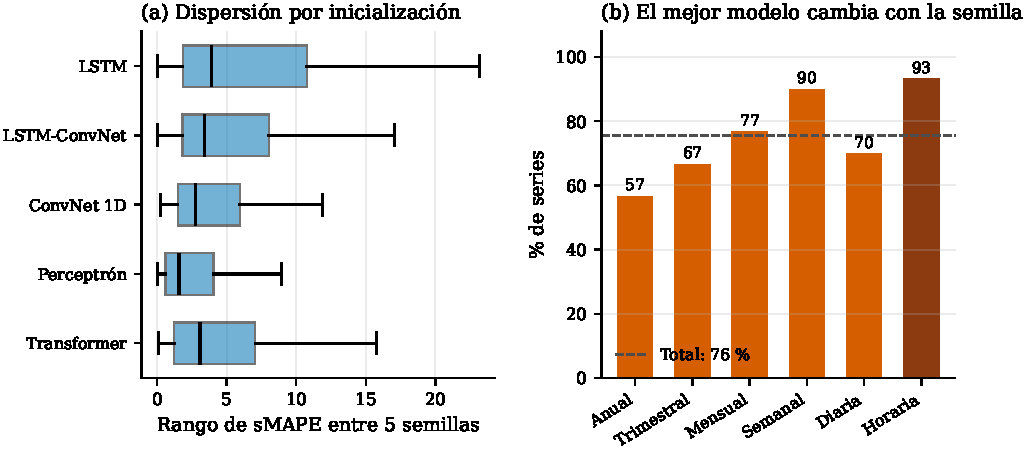
\includegraphics[width=\linewidth]{figuras/fig8_varianza_semillas.pdf}
\caption{(a) Distribution of the sMAPE range across five seeds, by architecture. (b)
Percentage of series in which the winning architecture changes when the seed changes. The
hourly frequency, highlighted, is the most unstable of the six despite being the only one
where the networks beat the benchmark.}
\label{fig:semillas}
\end{figure}

\begin{table}[htbp]
\centering
\caption{Stability of the ranking by frequency. The gap is the sMAPE difference between
the best and the second architecture; the noise is the median range across seeds.}
\label{tab:estabilidad}
\begin{tabular}{lrrrr}
\toprule
\textbf{Frequency} & \textbf{Winner changes} & \textbf{Gap 1st--2nd} & \textbf{Noise} & \textbf{Noise/gap} \\
\midrule
Hourly     & \textbf{93\%} & 0.41 & 2.25 & \textbf{5.5$\times$} \\
Weekly     & 90\% & 1.02 & 4.85 & 4.8$\times$ \\
Monthly    & 77\% & 0.94 & 2.68 & 2.8$\times$ \\
Daily      & 70\% & 0.40 & 1.01 & 2.5$\times$ \\
Quarterly  & 67\% & 1.61 & 3.87 & 2.4$\times$ \\
Yearly     & 57\% & 2.48 & 4.27 & 1.7$\times$ \\
\midrule
Total      & 76\% & 0.92 & 2.81 & 3.0$\times$ \\
\bottomrule
\end{tabular}
\end{table}

\paragraph{The instability is greatest where the networks work.}
Table~\ref{tab:estabilidad} contains the most uncomfortable result of the work. The hourly
frequency is the only one where neural architectures beat the benchmark
(Section~\ref{sec:horaria}, OWA between $0.76$ and $0.81$), and it is also \emph{the most
unstable of the six}: the winner changes in 93\% of the series and the initialization
noise is five times the gap between the first and the second.

The consequence is precise. In hourly series one may claim that \emph{the family} of
neural models is competitive, but not \emph{which architecture} is. A work reporting, from
a single run, that one architecture beats another on hourly data is reporting
initialization noise with high probability.

The pattern across frequencies does not follow sample size but the separation between
architectures: the frequencies where the gap between the first and the second is small
---hourly $0.41$, daily $0.40$, monthly $0.94$--- are those where the choice of the winner
is most fragile, regardless of how many observations each series has.

\paragraph{Averaging seeds does not solve selection.}\label{sec:ensamble}
The usual answer to initialization instability is to average several seeds. Two objectives
that practice pursues should be distinguished, because only one of them is solved that
way.

Averaging \emph{forecasts} reduces the error, and it is the classical reason for building
ensembles; that effect is not quantified here, because the experiment recorded the errors
per seed and not the predictions. Averaging \emph{scores} in order to decide which
architecture to use is a different objective, and that one was measured.

We compared the winning architecture that an experiment with $k$ seeds would yield against
the one another independent experiment with $k$ different seeds would yield. With a single
seed, two experiments agree in 52.6\% of the cases (1{,}800 comparisons). With two
averaged seeds, in 60.8\% (2{,}700 comparisons). The improvement is eight points and the
result is still close to chance.

The reason is one of scale. The standard deviation of the average decreases as
$1/\sqrt{k}$, but it starts from 1.18 sMAPE points, while the median gap between the first
and the second architecture is 0.92 points. With five seeds, the expected difference
between two independent experiments is still 80\% of that gap. Reaching a noise level
equal to half the gap would require on the order of thirteen seeds per series and
architecture.

The operational conclusion is not that ensembles are useless ---they reduce forecast
error, which is a real benefit not measured here--- but that \textbf{with a realistic
budget of initializations, the best architecture for a given series is not identifiable}.
Faced with that, two positions are defensible: combining architectures instead of choosing
one, or choosing the most stable one ---the perceptron, with a coefficient of variation of
6.2\%--- and accepting the 0.33 sMAPE points it concedes to the Transformer.

\paragraph{Fixing the seed is not enough to reproduce.} The three frequencies of the
preliminary experiment were re-run with the same series and the same seeds, expecting
exact reproduction. \textbf{None of the 2{,}250 shared measurements repeats}; the maximum
difference in sMAPE reaches $105.8$. The cause is not the seed but the environment: the
preliminary run used four compute threads and the definitive one two, and without enabling
operation-level determinism the order of floating-point reduction depends on the number of
threads.

The aggregate statistic, by contrast, does reproduce: the percentage of series in which
the winner changes goes from 68\% to 67\% over the same three frequencies. One point of
difference. \emph{No individual measurement survives the re-run; the conclusion does.}

This reinforces the argument rather than weakening it and adds a recommendation to the
reporting protocol: reporting the seed is insufficient, one must also declare the number
of threads and the determinism configuration, and the results must be read as statistics
over many series and not as point measurements.


% =====================================================================
\section{Discussion}\label{sec:discusion}
% =====================================================================

\paragraph{From correlation to decision.} The natural objection to a descriptive index is
that correlating is not serving, and much of the time series feature literature does not
answer it. Section~\ref{sec:enrutamiento} answers it as it should be answered: with a rule
learned on some series and evaluated on others. The contribution is modest in magnitude
---it closes 10.5\% of the distance to the attainable optimum--- but consistent,
significant and incremental with respect to the \emph{right control}: any work proposing a
stratification criterion should compare itself against frequency and not against a single
model, which is too weak a rival. The scalar does not exhaust the problem either: the best
policy over the 29 attributes closes 15.0\% (Section~\ref{sec:meta}), so that the index
obtains seven tenths of what the full apparatus achieves at a fraction of the cost of
maintaining it.

\paragraph{Stratify before modeling.} The mechanism is the one that motivated the initial
hypothesis: the internal structure of a series, measured before fitting any model,
anticipates forecasting difficulty. The factor of 3.29 between extreme quartiles and the
116\% difference between groups make it possible to allocate computational budget
differentially, reserving expensive methods for where they can make a difference. That the
optimal routing granularity coincides with the cardinality found by geometric criteria
---though not with its boundary--- suggests that binariness is a property of the
collection and not an artifact of the procedure.

\paragraph{Stratification must be within frequency.} The observed dependence ---from
$r=0.736$ to $r=0.019$--- implies that applying a single complexity threshold over the
aggregate collection would be a mistake. The index works as a stratification criterion
within each frequency, not across them.

\paragraph{A frequency without structure.} The daily case suggests a more general
conclusion: there exist collections for which the search for a better model has zero
return. The strongest evidence in that direction comes not from this work but from the
competition itself: the official results show that \emph{both the winning method and the
runner-up lose against Naive2 on the daily series} (Section~\ref{sec:frecuencia}). Two
systems built by specialized teams, evaluated blind, fall behind a deseasonalized random
walk in an entire frequency. That the index does not discriminate there ceases to be a
weakness and becomes a correct diagnosis: detecting it in advance avoids an expense no
method will recover.

\paragraph{The ceiling, and where it comes from.} The most useful result of this work is
not that the index works but how much it works, and against which alternative. The
superiority of combination over selection has been established for half a century
\cite{bates1969,wang2023} and is not claimed here; what these pages add is placing it on
the same scale as structural characterization, on the same data and protocol. The
index-based rule closes 10.5\% of the distance to the per-series oracle and the best
policy over the 29 attributes 15.0\%: the remaining 85\% is reached by neither.
\textbf{The limit is not imposed by having summarized structure in a scalar: it is imposed
by feature-based model selection as an approach}, and whoever seeks to close that 85\%
will not do so by refining the attribute vector. Section~\ref{sec:m3} confirms this
outside M4, where the unclosed fraction reaches 93.3\%.

The cause is identifiable. The classifier that predicts \emph{which} model wins is right
in only 18.5\% of the series (Section~\ref{sec:meta}), and the winning neural architecture
changes with the seed in 76\% of them (Section~\ref{sec:semillas}): the decision rests on
an unstable signal, because the candidates are separated by less than the noise of the
measurement itself. Hence a concrete design recommendation: \textbf{it is advisable to
decide on the expected error of each candidate and not on which of them will win}. The
reason is not that the label is noise ---both formulations share that label--- but that
predicting the winner and trusting it discards the cost structure, and that structure is
extreme: the worst 1\% of the series concentrates 40\% of the damage. With the loss
corrected and nothing else touched, the same classifier goes from OWA 1.493 to 0.866 and
places ahead of the regression policy (0.875).

\paragraph{Reproducibility of neural rankings.} The result of
Section~\ref{sec:semillas} has reach beyond this work: if in 76\% of the series the
winning architecture depends on the seed ---and in 93\% in the frequency where those
architectures actually work--- fine-grained rankings that do not report variance across
initializations are not interpretable.

To this is added that fixing the seed turned out to be insufficient for reproduction: on
varying the number of compute threads, none of the 2{,}250 repeated measurements agreed,
even though the aggregate statistic stayed within one percentage point. The practical
recommendation is twofold: declare seed, number of threads and determinism configuration,
and report dispersion across initializations as part of the standard protocol. A third one
---averaging several seeds--- turns out to be less favorable than is usually assumed
(Section~\ref{sec:ensamble}).

\paragraph{Implications for production systems.} The distinction between mediocre failure
and catastrophic failure (Section~\ref{sec:extremos}) is decisive for deployment: a system
serving automatic forecasts should incorporate a plausibility bound ---rejecting those
that depart from the historical range by more than a multiple of the interquartile
range--- before exposing the result.


% =====================================================================
\section{Limitations}\label{sec:limitaciones}
% =====================================================================

\begin{enumerate}
\item \textbf{Coverage of the feature vector.} 65 weekly series are discarded for
      insufficient length, so that the structural analyses cover 99{,}935 of 100{,}000
      series. The loss concentrates in the frequency with the smallest sample size.

\item \textbf{Fixed orders in the statistical models.} ARIMA and SARIMA are fitted with
      orders $(1,1,1)$ and $(1,1,1)(1,1,1)_m$ without automatic selection. The choice is
      deliberate ---a homogeneous measure of difficulty is sought, not the best model per
      series--- but it implies that the reported OWA values are lower bounds on attainable
      performance.

\item \textbf{Size of the model evaluation.} The bank was evaluated on 5{,}773 series and
      not on the 100{,}000, for computational cost. The samples are random within each
      frequency, with stratification by category in yearly and monthly. The imbalance
      matters where one weights by population: the monthly frequency weighs 48\% of the
      collection and contributes 1{,}000 evaluated series out of 48{,}000, that is 2.1\%.
      We checked what correcting it would change: setting the sampling error of that
      frequency to zero in the bootstrap ---the limit of evaluating it in full--- the
      interval of Section~\ref{sec:nbeats} narrows from $0.023$ to $0.017$ and still
      contains zero: the imbalance is real but it is not what sustains that tie. The
      yearly frequency was indeed enlarged, from 1{,}000 to 2{,}000 series, as the one
      contributing most to the uncertainty between policies; the effect was to narrow the
      intervals without altering any verdict, except to make visible that the difference
      between combining and stratifying had never been significant.

\item \textbf{Scope of the seed experiment.} The variance by initialization was measured
      on 180 series, 30 of each frequency. The qualitative result ---the winner changes---
      was reproduced in an independent re-run within one percentage point, but the exact
      percentages carry the uncertainty of that sample.

\item \textbf{Seasonal period in the quarterly frequency.} The recorded configuration
      reveals that ARIMA and SARIMA were fitted on the quarterly series with $m=12$
      instead of $m=4$, due to a parameter that was not propagated. On a subsample of 50
      series the mean sMAPE goes from $9.231$ to $9.421$, automatic order selection
      produces the same model in 23 of the 50, and the difference is not significant
      (paired Wilcoxon, $p=0.97$). It is documented for transparency; the conclusions do
      not depend on it.

\item \textbf{Seasonality conventions.} Two frequencies were processed with $m=12$ in the
      construction of lags before aligning the pipeline with the official M4 definition.
      The structural results do not depend on that choice; the stored forecast errors for
      those frequencies carry it.

\item \textbf{Sampling frame.} An intermediate file of the monthly frequency was truncated
      at $2^{14}$ series out of 48{,}000 and, since M4 orders by economic category, that
      block contained only two of the six. The sampling was redone in stratified form; it
      is documented because the draw was correct and the bias came from the frame, with no
      alarm observable in the procedure.

\item \textbf{The model bank predates recent neural architectures.} The four networks
      evaluated ---perceptron, 1D ConvNet, LSTM and Transformer--- are generic
      architectures trained series by series, and there are no global models designed for
      collections, such as N-BEATS \cite{oreshkin2020}. The claim that only six models
      beat the benchmark is conditional on this bank, and an updated one would modify
      which models make up the sets of Section~\ref{sec:combinar}. It would not change the
      comparison between policies, because they all operate on the same bank.

\item \textbf{N-BEATS does not converge in the monthly frequency.} With the
      implementation used, the model fails systematically in monthly (median sMAPE 31.3
      against 14.4 for the benchmark, in all five seeds). The failure is in the center of
      the distribution and not in the tail: these are not extreme cases but a model that
      does not learn. Since monthly concentrates 48\% of the collection, no global OWA is
      reported for N-BEATS. The effect on Section~\ref{sec:nbeats} is conservative: with
      an implementation that worked in all six frequencies, the optimal policy would move
      even closer to ``always use the same model'', which is the direction the result
      already points in.

\item \textbf{Asymmetry of training data.} N-BEATS is trained on all the series of each
      frequency while the candidates of the bank are fitted series by series on the
      evaluated sample. There is no leakage ---only the training portions are used--- but
      part of its advantage measures access to two orders of magnitude more series and not
      only the architecture.

\item \textbf{Indirect comparison with FFORMA.} Section~\ref{sec:meta} implements the
      \emph{approach} of FFORMS and FFORMPP on these data, not the published methods.
      FFORMA combines forecasts with learned weights and the available record keeps errors
      per series, not the predictions of its base ensemble; its published OWA moreover
      corresponds to a different set of series and a different pool of methods, so that it
      is not directly comparable with the figures of this work.

\item \textbf{What the split-based tests claim.} Several contrasts in this work ---paired
      Wilcoxon in Sections~\ref{sec:enrutamiento}, \ref{sec:dospasos} and in the
      comparison with catch22--- take the split as the unit. Thirty splits of the same
      5{,}674 series are not thirty independent samples, so those $p$ values measure
      \textbf{consistency under re-splitting the sample} and not population significance;
      read as the latter they would be anticonservative. The central claims of the work
      ---the contribution of the index by ensemble size, the comparison between combining
      and stratifying, and the regime of Section~\ref{sec:nbeats}--- rest instead on
      resampling of series, which is the correct unit for generalizing. The Friedman test
      of Section~\ref{sec:friedman} is unaffected: it blocks by series.

\item \textbf{External validity: the magnitudes are M4's, the mechanisms are not.}
      Section~\ref{sec:m3} repeats the protocol on M3 and the result must be stated in
      full: the ceiling and the diagnosis of the classifier do repeat ---there the best
      policy leaves 93.3\% of the gap unrecovered---, but \textbf{the 10.5\% that
      index-based routing closes falls to 1.9\%}, because the M3 bank is too homogeneous
      for there to be anything to distribute. The dispersion threshold at which the regime
      reverses was not replicated in any other collection. The magnitudes of this work
      must therefore be read as a measurement on M4 and its bank, not as constants of the
      problem; the mechanisms are indeed independent of the collection: that an unstable
      label cannot be learned, that a long-tailed loss requires deciding on expected cost
      and not on the most probable class, and that averaging cancels biases among
      comparable components and drags down the best one when one dominates.
\end{enumerate}


% =====================================================================
\section{Conclusions}\label{sec:conclusiones}
% =====================================================================

This work showed that a measure of structure computable before fitting any model does not
merely describe forecasting difficulty: it serves to decide. Assigning a model by
frequency and complexity stratum beats assigning it by frequency alone in all 30 splits
evaluated out of sample, and the optimal granularity ---two strata--- is the cardinality
the cluster analysis had identified on internal criteria, without observing any forecast
error. Two independent routes arrive at the exploitable structure being binary; not at the
same boundary, because the two partitions agree on 70.1\% of the series.

The central contribution, however, is not that but its measurement and its location. The
rule closes 10.5\% of the distance to the per-series oracle and the best policy over the
29 attributes 15.0\%: twenty-nine attributes buy seventeen thousandths of OWA over a
scalar with two strata and leave 85\% of the gap intact. \textbf{The ceiling is not
imposed by the scalar summary.} It is partly imposed by the decision to \emph{choose}:
averaging the five best of each stratum widens the closed fraction from 8.5\% to 14.4\%,
and that decision weighs as much as stratifying. That combining beats choosing is not a
finding of this work but of half a century of literature \cite{bates1969,wang2023}; what
is one is measuring both decisions on the same scale, and finding that knowing \emph{what}
to combine is worth 0.39 OWA points against drawing among the ten best.

That result has a scope the work delimits rather than leaves implicit. On adding a modern
global model to the bank, the regime reverses where that model dominates: in the four
frequencies where N-BEATS leads the runner-up by between 0.060 and 0.231 of OWA, choosing
one beats combining five and the contribution of the index ceases to be significant. That
the inversion does not reach the aggregate depends on the monthly frequency, 48\% of the
collection, being where the implementation used does not converge. A single mechanism
explains both regimes ---averaging cancels biases among equals and drags down the best one
when one dominates---, from which the operating recommendation follows: \textbf{look at
the quality spread of the pool before deciding between choosing and combining}. Within the
regime with no dominant model, the contribution of the index is greatest when choosing and
decays when combining until it is undetectable with three or more: characterization serves
precisely in the decision that pays least. It is the tension the work leaves open, and it
reconciles the measured ceiling with FFORMA's second place ---which combines instead of
choosing, so that its merit falls on the learned weights more than on the features---
rather than contradicting it.

The cause of the ceiling was identified, and corrected along the way. The label that
feature-based selection has to learn ---which method wins in this series--- is largely
noise: in 76\% of the series the winning neural architecture changes when only the
initialization changes, with a maximum of 93\% in the hourly frequency. But the failure of
the classifier, which ends up worse than not routing, is \emph{not} a consequence of that
noise: with the same label and the same forest, changing the decision rule from the most
probable class to minimum expected regret takes it from OWA $1.493$ to $0.866$. The design
recommendation holds ---predict the error of each candidate rather than predict which one
wins--- but because it encodes the loss and not because it dodges a noisy label. It is
accompanied by a reporting recommendation: fine-grained rankings among architectures that
do not report dispersion across seeds are not interpretable.

The replication on M3, with the published forecasts of 22 methods and the index
transferred without refitting, separates what belongs to the approach from what belongs to
M4. The ceiling holds and worsens ---93.3\% goes unrecovered there--- and the diagnosis of
the classifier repeats, even in a bank where no candidate diverges. The margin of
index-based routing, by contrast, falls from 10.5\% to 1.9\%, because five of the 22
methods fall within 5\% of the best: it is the heterogeneity of the bank, and not that of
the series, that sets how much there is to distribute. The index orders by difficulty in
both collections; only in one of them does that translate into a better choice of model.

The measure that makes all of the above possible is a structural complexity index over 29
descriptors of the 100{,}000 series: it correlates with the error of the naive forecast,
separates quartiles whose mean error differs by a factor of 3.29 and is not redundant with
the established measures. Its discriminating power depends strongly on the frequency,
which makes it necessary to stratify within each one. Daily is the instructive limiting
case: no measure discriminates and, consistently, no model beats the benchmark ---not even
the top two of the competition. An index without discriminating power in a collection is
actionable information, not a failure of the diagnosis. The bank under the official metric
confirms in addition that classical methods remain competitive ---only six beat Naive2,
the best with OWA $=0.936$--- and reveals the complete inversion of the ordering in the
hourly frequency; the Friedman test with Nemenyi post-hoc qualifies the ranking: a
statistical tie among ARIMA, SARIMA and ETS at the top, and hybrids whose problem is not
typical performance but tail risk.

The starting hypothesis ---group the series by structure and assign to each group the
method that suits it--- therefore turns out to be correct in its direction, modest in its
scope and wrong in its form: the partition structure admits is binary and not a taxonomy
of regimes, its contribution concentrates in the decision that pays least, and its
magnitude depends on the bank against which it is measured. Even so, the bulk of the
distance to the oracle goes unclosed ---a distance that bounds from above what is
recoverable and does not measure it, because it includes error no model in the bank could
have avoided.

\paragraph{Future work.} Three lines follow: incorporating the index as a decision
variable in an automatic selection system and measuring the gain against a uniform policy;
extending the evaluation to the full collection; and, since the replication on M3 showed
that the routing margin depends on the heterogeneity of the bank, measuring that
dependence directly ---varying the composition of the bank at a fixed collection--- rather
than continuing to change collections.


% =====================================================================
\section*{Code and data availability}
% =====================================================================

The data come from the M4 competition and are publicly accessible \cite{m4results}; those
of the external replication, from the published M3 forecasts \cite{mcomp}. The complete
code ---features, reduction, clustering, entropies, official metrics, evaluation of the
bank and the experiments on routing, meta-learning, combination and external
validation--- is at \url{https://github.com/JorgeChiles/m4-estructura-combinacion}, under
the MIT license, with the execution instructions in order and the dependencies pinned to
fixed versions. Re-running the deterministic stages reproduces everything exactly:
difference $0.00$ in the index of the 99{,}935 series, in the group assignments, in the
principal components, in the three entropies and in the errors of the statistical and
machine learning methods. The stochastic components ---the networks--- do not reproduce,
and that lack of reproducibility is reported as a result in
Section~\ref{sec:semillas} rather than omitted.


% =====================================================================
%  Bibliografia: identica a la del original salvo las dos anotaciones que
%  estaban en espanol. Mismas claves de \cite, mismo orden.
% =====================================================================
{\scriptsize
\begin{thebibliography}{99}
\setlength{\itemsep}{0pt}\setlength{\parskip}{0pt}
% =====================================================================

\bibitem{bates1969}
Bates, J. M., \& Granger, C. W. J. (1969). The combination of forecasts.
\emph{Operational Research Quarterly}, 20(4), 451--468.

\bibitem{wang2023}
Wang, X., Hyndman, R. J., Li, F., \& Kang, Y. (2023). Forecast combinations: an over
50-year review. \emph{International Journal of Forecasting}, 39(4), 1518--1547.

\bibitem{makridakis2020}
Makridakis, S., Spiliotis, E., \& Assimakopoulos, V. (2020).
The M4 Competition: 100,000 time series and 61 forecasting methods.
\emph{International Journal of Forecasting}, 36(1), 54--74.

\bibitem{makridakis2000}
Makridakis, S., \& Hibon, M. (2000). The M3-Competition: results, conclusions and
implications. \emph{International Journal of Forecasting}, 16(4), 451--476.

\bibitem{mcomp}
Hyndman, R. J. (2018). \emph{Mcomp: Data from the M-Competitions} [R package,
version 2.8]. Contains the 3,003 series of M3 and the forecasts of all participating
methods. \url{https://CRAN.R-project.org/package=Mcomp}

\bibitem{m4results}
M4 Team (2018). \emph{Evaluation and Ranks} [official results spreadsheet of the
M4 competition]. Mcompetitions/M4-methods repository.
\url{https://github.com/Mcompetitions/M4-methods}

\bibitem{smyl2020}
Smyl, S. (2020). A hybrid method of exponential smoothing and recurrent neural
networks for time series forecasting.
\emph{International Journal of Forecasting}, 36(1), 75--85.

\bibitem{wang2006}
Wang, X., Smith, K., \& Hyndman, R. (2006).
Characteristic-based clustering for time series data.
\emph{Data Mining and Knowledge Discovery}, 13(3), 335--364.

\bibitem{kang2017}
Kang, Y., Hyndman, R. J., \& Smith-Miles, K. (2017). Visualising forecasting algorithm
performance using time series instance spaces.
\emph{International Journal of Forecasting}, 33(2), 345--358.

\bibitem{fulcher2017}
Fulcher, B. D., \& Jones, N. S. (2017). hctsa: A computational framework for
automated time-series phenotyping using massive feature extraction.
\emph{Cell Systems}, 5(5), 527--531.

\bibitem{talagala2018}
Talagala, T. S., Hyndman, R. J., \& Athanasopoulos, G. (2023). Meta-learning how to
forecast time series. \emph{Journal of Forecasting}, 42(6), 1476--1501.

\bibitem{monteromanso2020}
Montero-Manso, P., Athanasopoulos, G., Hyndman, R. J., \& Talagala, T. S. (2020).
FFORMA: Feature-based forecast model averaging.
\emph{International Journal of Forecasting}, 36(1), 86--92.

\bibitem{oreshkin2020}
Oreshkin, B. N., Carpov, D., Chapados, N., \& Bengio, Y. (2020). N-BEATS: Neural basis
expansion analysis for interpretable time series forecasting.
\emph{International Conference on Learning Representations (ICLR)}.

\bibitem{lubba2019}
Lubba, C. H., Sethi, S. S., Knaute, P., Schultz, S. R., Fulcher, B. D., \& Jones, N. S.
(2019). catch22: CAnonical Time-series CHaracteristics.
\emph{Data Mining and Knowledge Discovery}, 33(6), 1821--1852.

\bibitem{bandt2002}
Bandt, C., \& Pompe, B. (2002). Permutation entropy: a natural complexity measure
for time series. \emph{Physical Review Letters}, 88(17), 174102.

\bibitem{richman2000}
Richman, J. S., \& Moorman, J. R. (2000). Physiological time-series analysis using
approximate entropy and sample entropy.
\emph{American Journal of Physiology --- Heart and Circulatory Physiology},
278(6), H2039--H2049.

\bibitem{lempel1976}
Lempel, A., \& Ziv, J. (1976). On the complexity of finite sequences.
\emph{IEEE Transactions on Information Theory}, 22(1), 75--81.

\bibitem{demsar2006}
Dem\v{s}ar, J. (2006). Statistical comparisons of classifiers over multiple data
sets. \emph{Journal of Machine Learning Research}, 7, 1--30.

\bibitem{talagala2019}
Talagala, T. S., Li, F., \& Kang, Y. (2022). FFORMPP: Feature-based forecast model
performance prediction.
\emph{International Journal of Forecasting}, 38(3), 920--943.

\bibitem{vanzyl2023}
van Zyl, T. L. (2023). Late meta-learning fusion using representation learning for
time series forecasting. \emph{arXiv preprint}. DOI: 10.48550/arXiv.2303.11000

\bibitem{vaiciukynas2021}
Vaiciukynas, E., Danenas, P., Kontrimas, V., \& Butleris, R. (2021). Two-step
meta-learning for time-series forecasting ensemble. \emph{IEEE Access}, 9,
62687--62696.

\bibitem{abdallah2025}
Abdallah, M., Rossi, R. A., Mahadik, K., Kim, S., Zhao, H., \& Bagchi, S. (2025).
Evaluation-free time-series forecasting model selection via meta-learning.
\emph{ACM Transactions on Knowledge Discovery from Data}, 19(3), 64:1--64:41.

\bibitem{digangi2022}
Di Gangi, L. (2022). Sparse convex combinations of forecasting models by meta
learning. \emph{Expert Systems with Applications}, 200, 116938.

\bibitem{raubitzek2021}
Raubitzek, S., \& Neubauer, T. (2021). Combining measures of signal complexity and
machine learning for time series analysis: A review. \emph{Entropy}, 23(12), 1672.
DOI: 10.3390/e23121672

\bibitem{huang2019}
Huang, Y., \& Fu, Z. (2019). Enhanced time series predictability with well-defined
structures. \emph{Theoretical and Applied Climatology}, 138(1--2), 373--385.

\bibitem{manero2021}
Manero, J., \& Béjar, J. (2021). Forecastability measures that describe the
complexity of a site for deep learning wind predictions.
\emph{Supercomputing Frontiers and Innovations}, 8(1), 8--27.

\bibitem{kovantsev2020}
Kovantsev, A., \& Gladilin, P. (2020). Analysis of multivariate time series
predictability based on their features. \emph{IEEE International Conference on Data
Mining Workshops (ICDMW)}, 348--355.

\bibitem{gundersen2023}
Gundersen, O. E., Shamsaliei, S., Kj\ae{}rnli, H. S., \& Langseth, H. (2023). On reporting robust and
trustworthy conclusions from model comparison studies involving neural networks and
randomness. \emph{ACM Conference on Reproducibility and Replicability}, 37--61.

\bibitem{agathangelou2020}
Agathangelou, P., Trihinas, D., \& Katakis, I. (2020). A multi-factor analysis of
forecasting methods: A study on the M4 competition. \emph{Data}, 5(2), 41.
DOI: 10.3390/data5020041

\bibitem{ingel2020}
Ingel, A., Shahroudi, N., Kängsepp, M., Tättar, A., Komisarenko, V., \& Kull, M.
(2020). Correlated daily time series and forecasting in the M4 competition.
\emph{International Journal of Forecasting}, 36(1), 121--128.

\bibitem{hyndman2006}
Hyndman, R. J., \& Koehler, A. B. (2006).
Another look at measures of forecast accuracy.
\emph{International Journal of Forecasting}, 22(4), 679--688.

\end{thebibliography}
}
